\documentclass[beamer=true]{standalone}
\usepackage[]{preamblesnotes}

\begin{document}
\settitle{透鏡\\Lenses}{光學第四課(II)}{周末班}

\begin{frame}
    {實像 Real images}
    \begin{columns}
        \column{.5\textwidth}
        \begin{itemize}
            \setlength{\itemsep}{.6em}
            \item 倒置。\\Inverted.
            \item 實像和物體在相反的一側。\\Image and object at opposite sides.
            \item 折射的光線通過實像。\\Refracted rays passes through image.
            \item 可以在屏幕上形成。\\Can form on screen.
            \item 可以用肉眼或相機觀察。\\Can be observed by naked eye or camera.
                  % \item 要看到清晰的像,觀察者的距離固定。\\The location of the observer is fixed to observe clear image.
        \end{itemize}
        \column{.5\textwidth}
        \begin{figure}
            \centering
            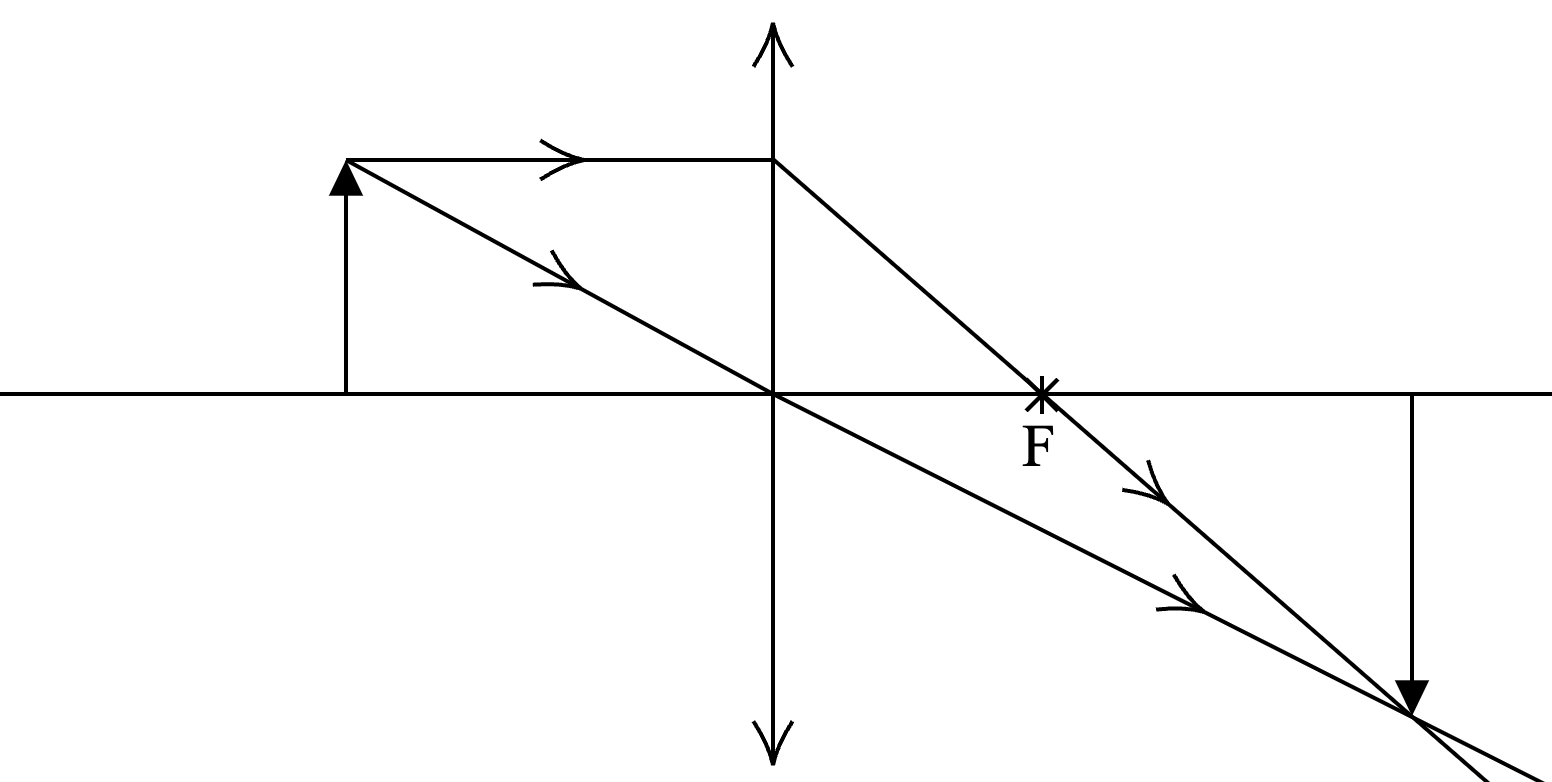
\includegraphics[width=\linewidth]{assets/x1eni1me.png}
        \end{figure}\bigskip
        \begin{itemize}
            \item 要看到清晰的像,觀察者的距離固定。\\The location of the observer is fixed to observe clear image.
        \end{itemize}
    \end{columns}



\end{frame}

\begin{frame}{虛像Virtual images}
    \begin{columns}
        \column{.5\textwidth}
        \begin{itemize}
            \setlength{\itemsep}{.6em}
            \item 必須是直立的。\\Must be erect.
            \item 虛像和物體在同一側。\\Image and object at same side.
            \item 折射的光線不會通過虛像。Refracted rays does not pass through image.
            \item 無法在屏幕上形成。\\Cannot form on screen.
            \item 可以用肉眼或相機觀察到清晰的像,觀察者的距離不需固定。\\Clear image can be observed by naked eye or camera, and location of the observer is not fixed.
        \end{itemize}
        \column{.5\textwidth}
        \begin{figure}
            \centering
            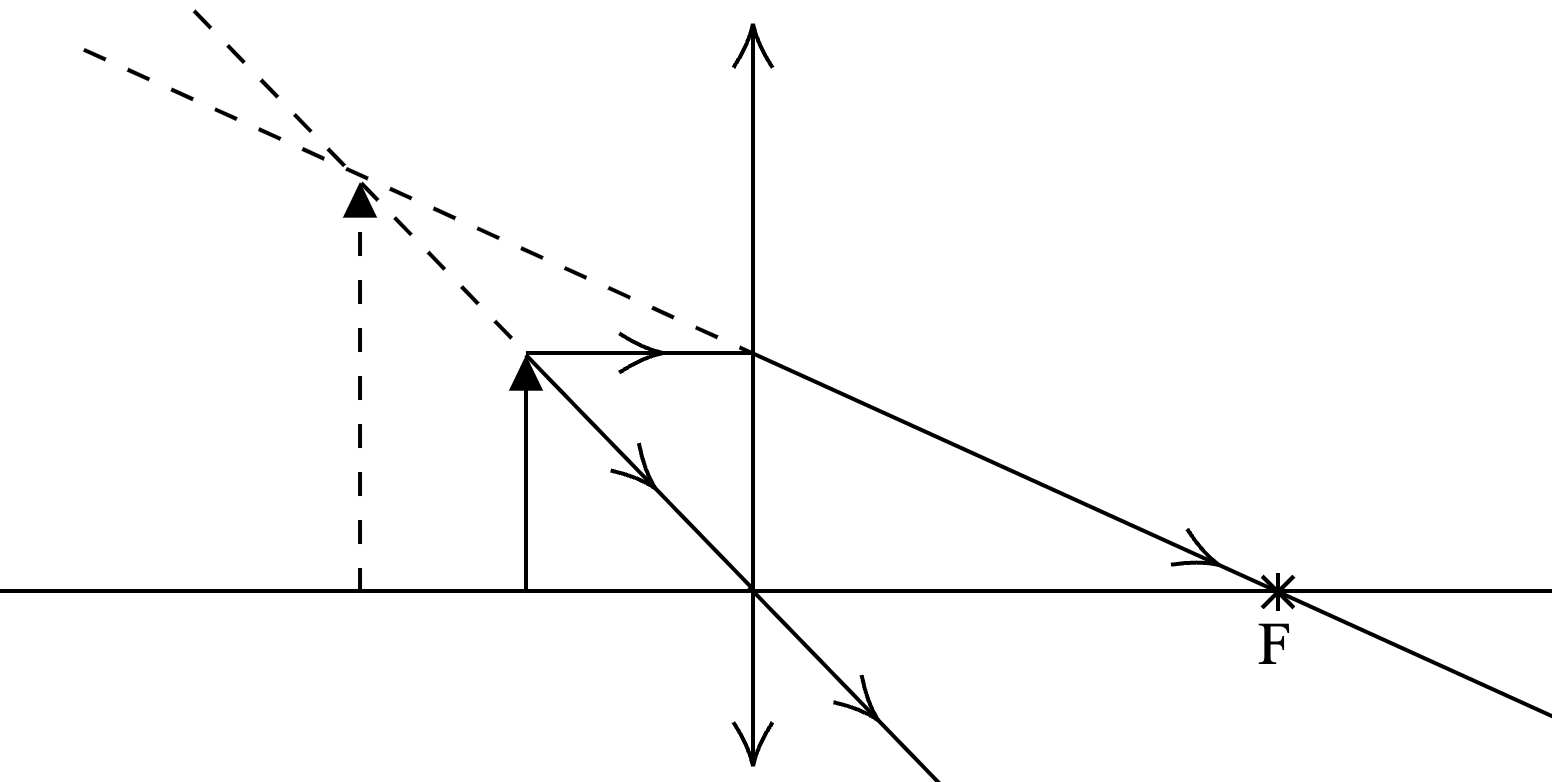
\includegraphics[width=1\linewidth]{assets/unxu9d32.png}
        \end{figure}\bigskip
        \begin{figure}
            \centering
            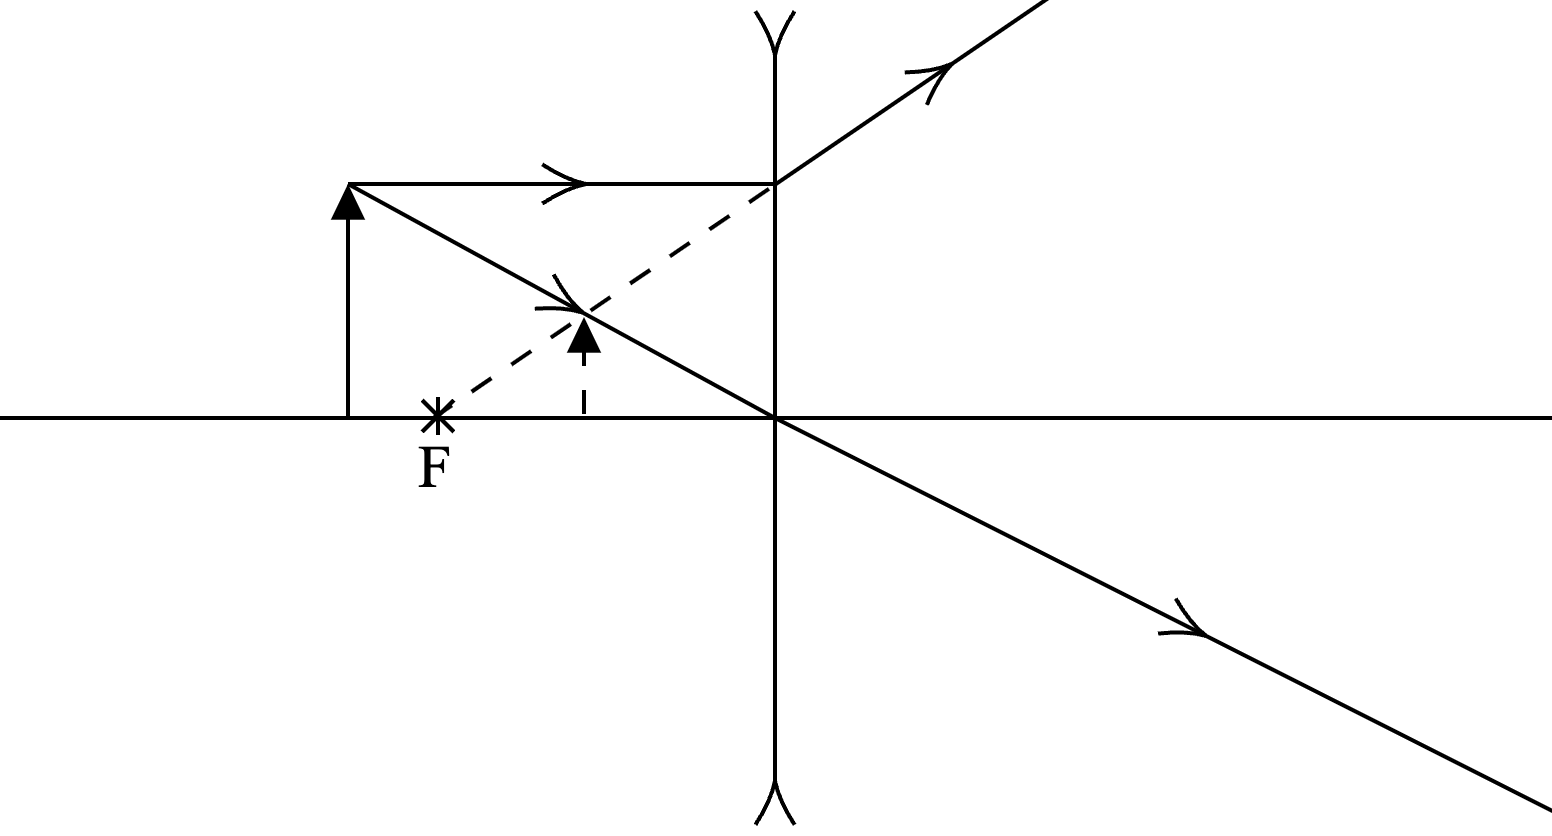
\includegraphics[width=\linewidth]{assets/dn1d33d.png}
        \end{figure}
        %         \bigskip
        % \begin{itemize}
        %     \item 要看到清晰的像,觀察者的距離不需固定。\\The location of the observer is not fixed to observe clear image.
        % \end{itemize}

    \end{columns}
\end{frame}

\begin{frame}
    {Identification of the lens 辨別透鏡}
    \par{\par\centering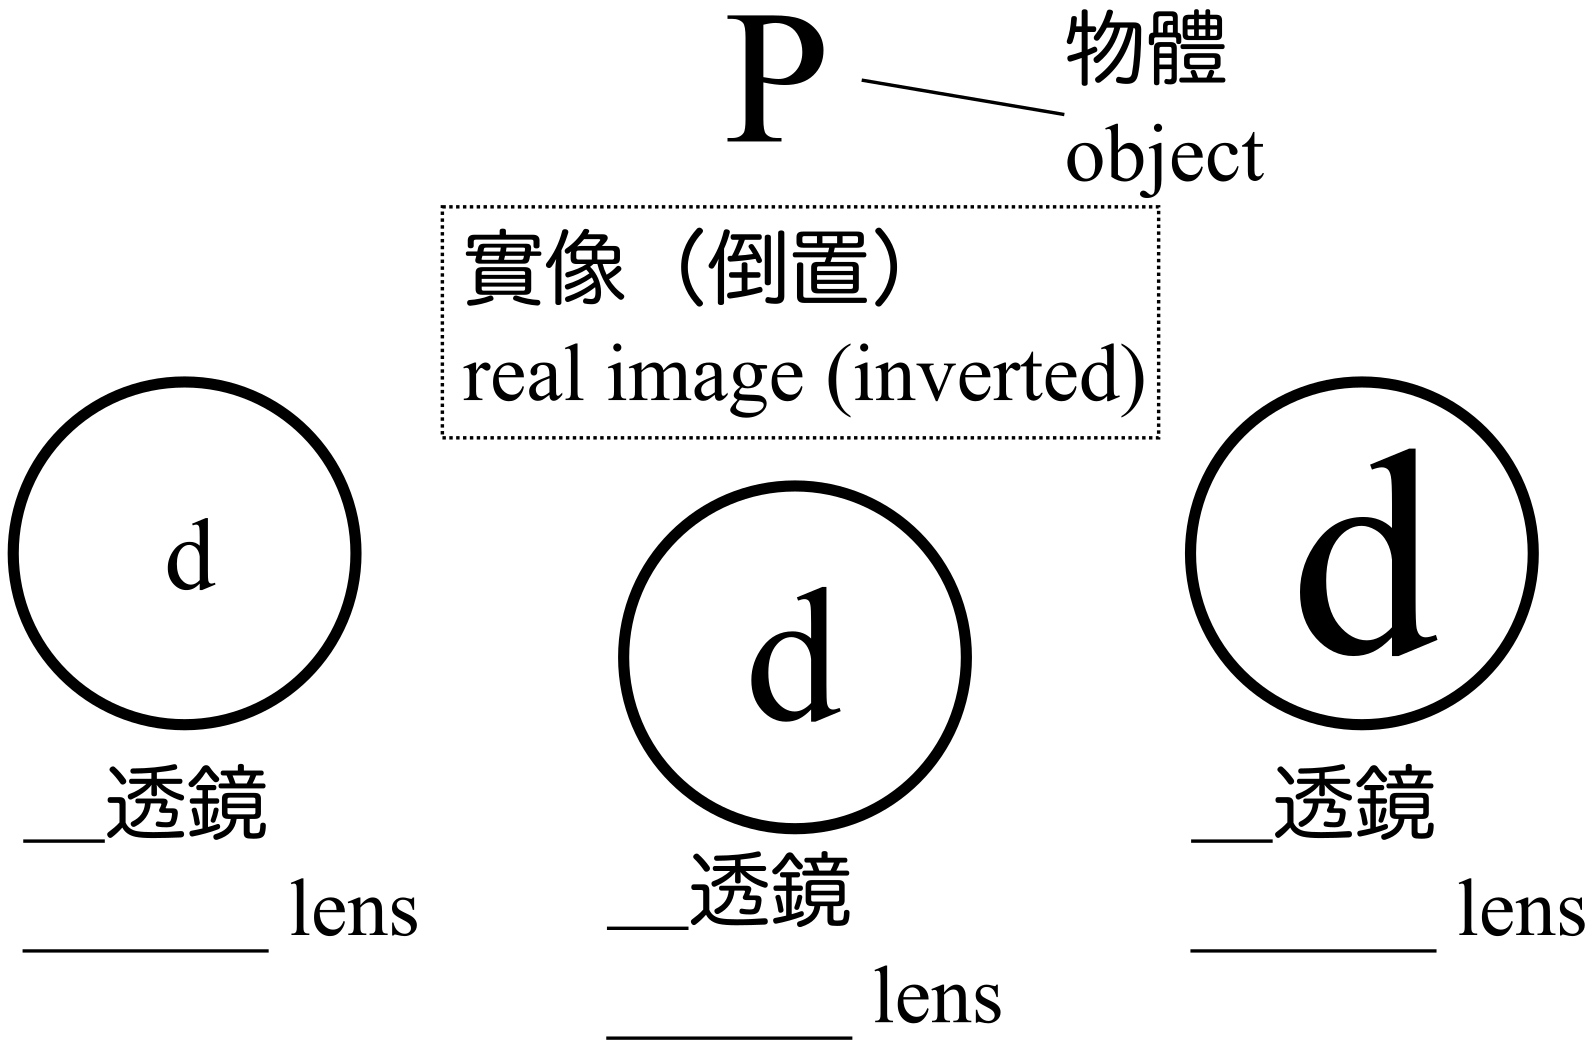
\includegraphics[width=\textwidth]{assets/1133445.png}\par}
\end{frame}
\begin{frame}
    {Identification of the lens辨別透鏡}
    % \par{\par\centering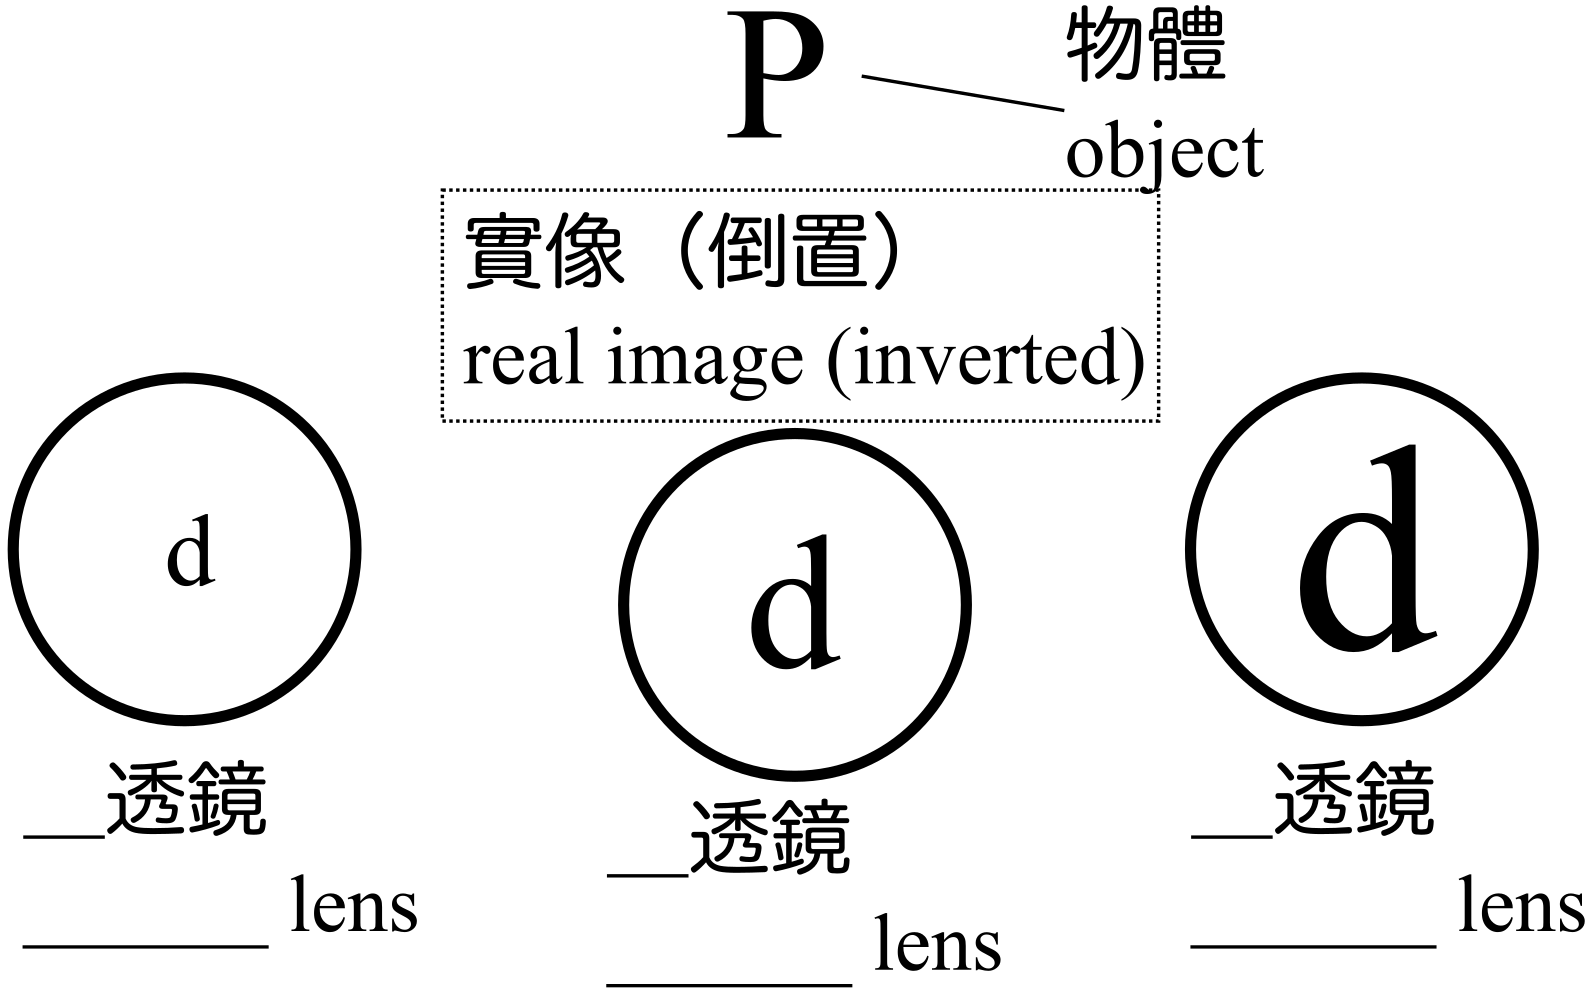
\includegraphics[width=\textwidth]{assets/ch5_2024-04-01-17-58-45.png}\par}
    \begin{figure}
        \centering
        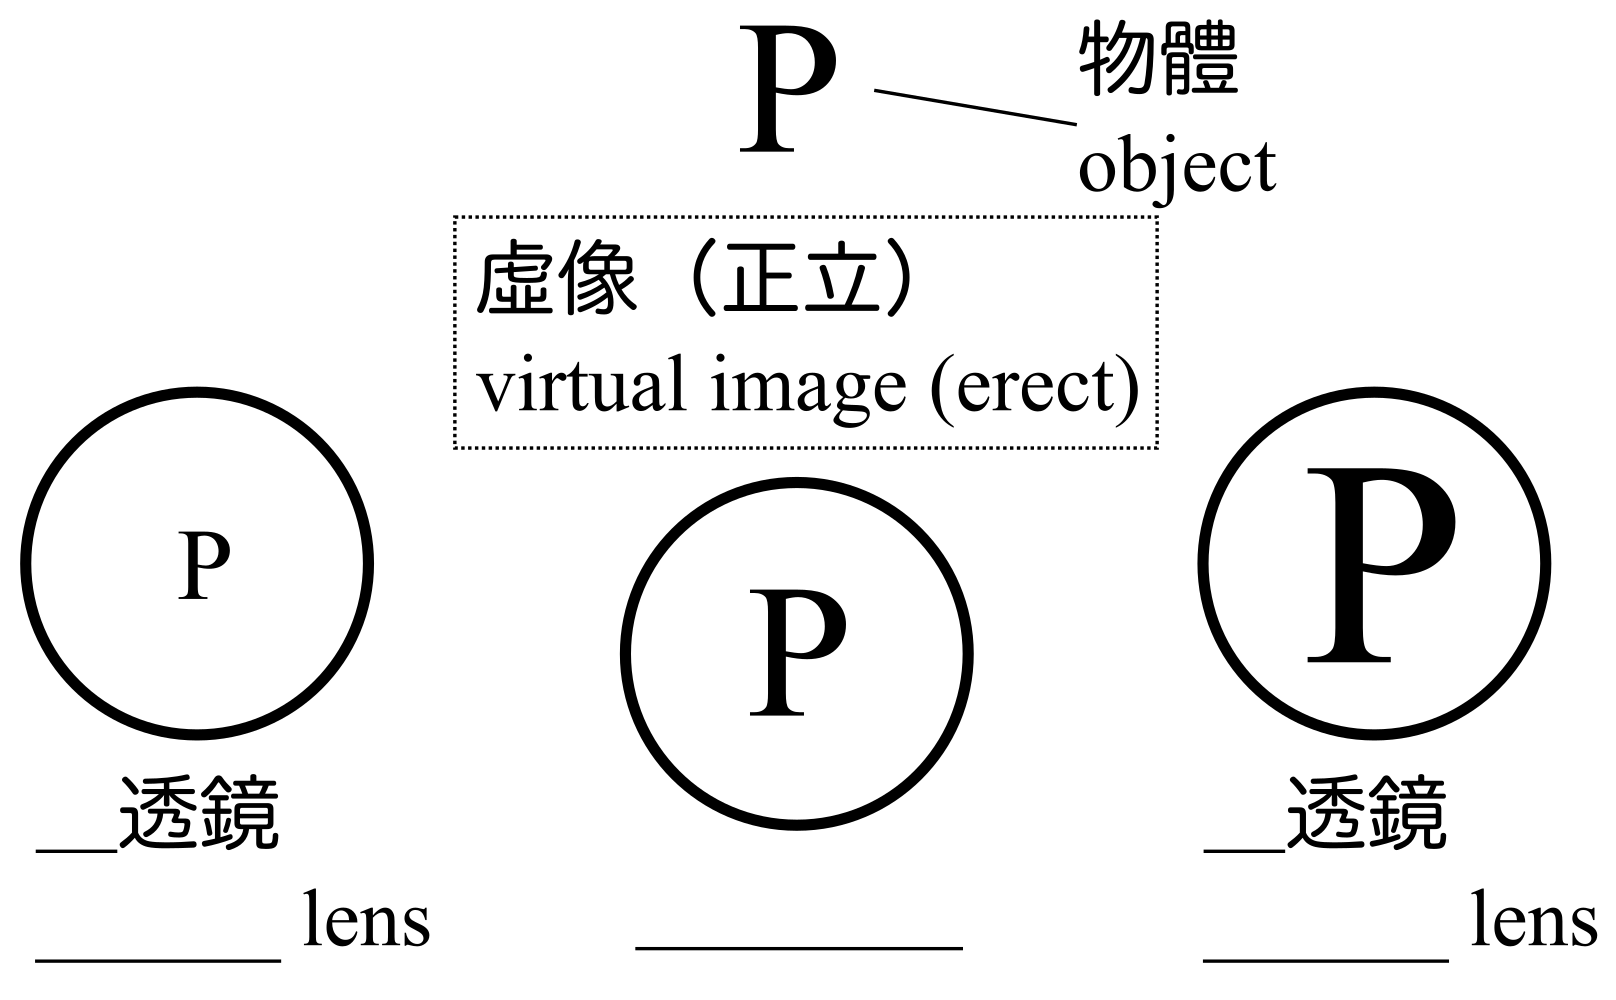
\includegraphics[width=1\linewidth]{assets/dedn2189u328n2.png}
    \end{figure}
\end{frame}

\begin{eg}
    一塊透鏡產生一個正立的成像。以下哪些敍述必定是正確的?\\An erect image is formed by a lens. Which of the following statements must be correct?
    \begin{statements}[before-skip=0pt,after-skip = 0pt]
        \task 成像是個虛像。\\The image is virtual.
        \task 該透鏡是一塊凹透鏡。\\The lens is a concave lens.
        \task 成像和物件均位於透鏡的同一方。\\The image and the object are on the same side of the lens.
    \end{statements}
    \begin{tasks}(2)
        \task (1)
        \task (1) \& (3)
        \task (2) \& (3)
        \task (1), (2) \& (3)
    \end{tasks}
\end{eg}

\begin{eg}
    \begin{figure}
        \centering
        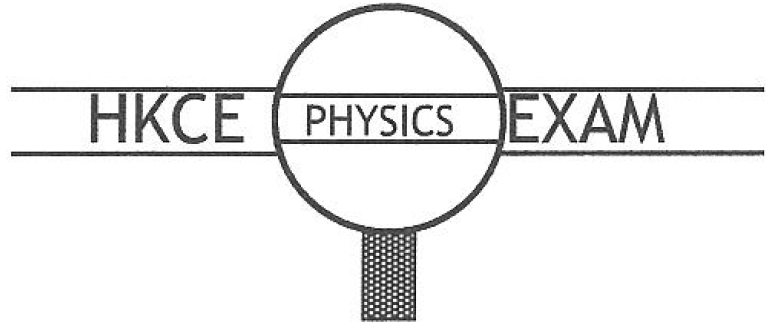
\includegraphics[width=0.5\linewidth]{assets/x8neu983eu23.png}


    \end{figure}
    一個透鏡被用來觀察紙上的一些文字。上方顯示了單字「PHYSICS」的成像。以下哪些陳述是正確的?\\A lens is used to look at some print on a paper. The image of the word ``PHYSICS'' is shown above. Which of the following statements is/are true?

\end{eg}
\begin{eg}
    \begin{statements}[before-skip=0pt,after-skip = 0pt]
        \task 該透鏡是一個會聚透鏡。\\The lens is a converging lens.
        \task 成像位於紙張和透鏡之間。\\The image lies between the paper and the lens.
        \task 成像是實像。\\The image is real.
    \end{statements}
    \begin{tasks}(2)
        \task 只有 (2)
        \task 只有 (1) 和 (2)
        \task 只有 (1) 和 (3)
        \task (1), (2) 和 (3)
    \end{tasks}
    \begin{tasks}(2)
        \task (2) only
        \task (1) and (2) only
        \task (1) and (3) only
        \task (1), (2) and (3)
    \end{tasks}
\end{eg}

\begin{eg}
    一位學生將一個透鏡放在一塊寫有「TEST」字樣的紙上,這是什麼透鏡?如果學生將透鏡從紙上移開更遠,成像的大小會有什麼變化?\\A student puts a lens at a certain distance above a paper with the word ``TEST'' written on it as shown in the figure. What is the lens? If the student moves the lens further away from the paper, what will be the change in the size of the image?
    % \bigskip
    \begin{figure}
        \centering
        
\includegraphics[width=0.5\linewidth]{assets/98n9du892nd923.png}
    \end{figure}
    \begin{tasks}[item-indent=2em,label-offset=0em,before-skip=0em,after-item-skip=.8em](2)
        \task [] \textbf{透鏡類型lens}
        \task [] \textbf{成像的大小變化\\change in size of image}
        \task [] \rule{1.5in}{.5pt}
        \task [] \rule{1.5in}{.5pt}
    \end{tasks}
\end{eg}

\begin{frame}{放大率Magnification}
    % \begin{figure}
    %     \centering
    %     \tikzset{every picture/.style={line width=0.75pt}} %set default line width to 0.75pt        

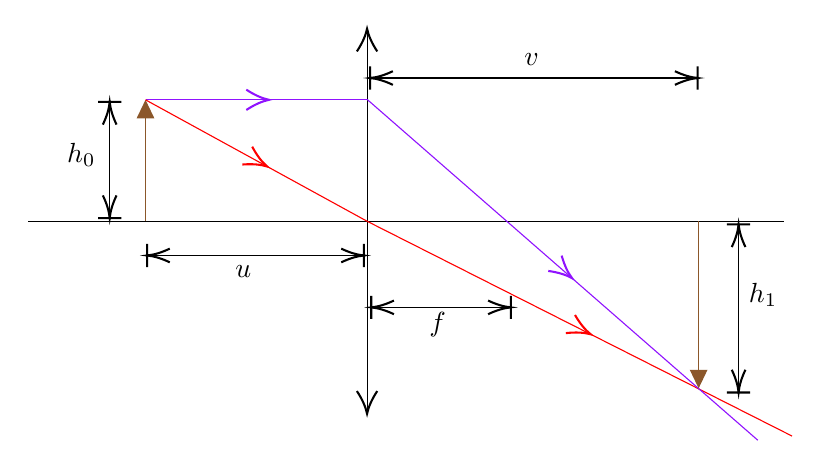
\begin{tikzpicture}[x=0.75pt,y=0.75pt,yscale=-1,xscale=1]
%uncomment if require: \path (0,1383); %set diagram left start at 0, and has height of 1383

%Straight Lines [id:da588141719156511] 
\draw    (176,797.75) -- (540,797.75) ;
%Straight Lines [id:da03250675150670723] 
\draw    (339.25,888.5) -- (339.25,707) ;
\draw [shift={(339.25,705)}, rotate = 90] [color={rgb, 255:red, 0; green, 0; blue, 0 }  ][line width=0.75]    (10.93,-4.9) .. controls (6.95,-2.3) and (3.31,-0.67) .. (0,0) .. controls (3.31,0.67) and (6.95,2.3) .. (10.93,4.9)   ;
\draw [shift={(339.25,890.5)}, rotate = 270] [color={rgb, 255:red, 0; green, 0; blue, 0 }  ][line width=0.75]    (10.93,-4.9) .. controls (6.95,-2.3) and (3.31,-0.67) .. (0,0) .. controls (3.31,0.67) and (6.95,2.3) .. (10.93,4.9)   ;
%Straight Lines [id:da6599102272548933] 
\draw [color={rgb, 255:red, 139; green, 87; blue, 42 }  ,draw opacity=1 ]   (232.5,797.75) -- (232.5,742.25) ;
\draw [shift={(232.5,739.25)}, rotate = 90] [fill={rgb, 255:red, 139; green, 87; blue, 42 }  ,fill opacity=1 ][line width=0.08]  [draw opacity=0] (8.93,-4.29) -- (0,0) -- (8.93,4.29) -- cycle    ;
%Straight Lines [id:da3477945298452818] 
\draw [color={rgb, 255:red, 144; green, 19; blue, 254 }  ,draw opacity=1 ]   (232.5,739.25) -- (339.5,739.25) ;
\draw [shift={(292,739.25)}, rotate = 180] [color={rgb, 255:red, 144; green, 19; blue, 254 }  ,draw opacity=1 ][line width=0.75]    (10.93,-4.9) .. controls (6.95,-2.3) and (3.31,-0.67) .. (0,0) .. controls (3.31,0.67) and (6.95,2.3) .. (10.93,4.9)   ;
%Straight Lines [id:da8220603631709424] 
\draw [color={rgb, 255:red, 255; green, 0; blue, 0 }  ,draw opacity=1 ]   (232.5,739.25) -- (339.25,797.75) ;
\draw [shift={(291.14,771.38)}, rotate = 208.72] [color={rgb, 255:red, 255; green, 0; blue, 0 }  ,draw opacity=1 ][line width=0.75]    (10.93,-4.9) .. controls (6.95,-2.3) and (3.31,-0.67) .. (0,0) .. controls (3.31,0.67) and (6.95,2.3) .. (10.93,4.9)   ;
%Straight Lines [id:da9703159868320685] 
\draw [color={rgb, 255:red, 255; green, 0; blue, 0 }  ,draw opacity=1 ]   (339.25,797.75) -- (544,901.25) ;
\draw [shift={(446.98,852.21)}, rotate = 206.82] [color={rgb, 255:red, 255; green, 0; blue, 0 }  ,draw opacity=1 ][line width=0.75]    (10.93,-4.9) .. controls (6.95,-2.3) and (3.31,-0.67) .. (0,0) .. controls (3.31,0.67) and (6.95,2.3) .. (10.93,4.9)   ;
%Straight Lines [id:da7461655834059451] 
\draw [color={rgb, 255:red, 144; green, 19; blue, 254 }  ,draw opacity=1 ]   (339.5,739.25) -- (527.5,903.25) ;
\draw [shift={(438.02,825.19)}, rotate = 221.1] [color={rgb, 255:red, 144; green, 19; blue, 254 }  ,draw opacity=1 ][line width=0.75]    (10.93,-4.9) .. controls (6.95,-2.3) and (3.31,-0.67) .. (0,0) .. controls (3.31,0.67) and (6.95,2.3) .. (10.93,4.9)   ;
%Straight Lines [id:da3379496419254937] 
\draw [color={rgb, 255:red, 139; green, 87; blue, 42 }  ,draw opacity=1 ]   (499,797.75) -- (499,875.25) ;
\draw [shift={(499,878.25)}, rotate = 270] [fill={rgb, 255:red, 139; green, 87; blue, 42 }  ,fill opacity=1 ][line width=0.08]  [draw opacity=0] (8.93,-4.29) -- (0,0) -- (8.93,4.29) -- cycle    ;
%Straight Lines [id:da6356533316132849] 
\draw    (233.25,814.25) -- (337.75,814.25) ;
\draw [shift={(337.75,814.25)}, rotate = 180] [color={rgb, 255:red, 0; green, 0; blue, 0 }  ][line width=0.75]    (0,5.59) -- (0,-5.59)(10.93,-3.29) .. controls (6.95,-1.4) and (3.31,-0.3) .. (0,0) .. controls (3.31,0.3) and (6.95,1.4) .. (10.93,3.29)   ;
\draw [shift={(233.25,814.25)}, rotate = 0] [color={rgb, 255:red, 0; green, 0; blue, 0 }  ][line width=0.75]    (0,5.59) -- (0,-5.59)(10.93,-3.29) .. controls (6.95,-1.4) and (3.31,-0.3) .. (0,0) .. controls (3.31,0.3) and (6.95,1.4) .. (10.93,3.29)   ;
%Straight Lines [id:da2133877127707755] 
\draw    (340.75,728.75) -- (498.5,728.75) ;
\draw [shift={(498.5,728.75)}, rotate = 180] [color={rgb, 255:red, 0; green, 0; blue, 0 }  ][line width=0.75]    (0,5.59) -- (0,-5.59)(10.93,-3.29) .. controls (6.95,-1.4) and (3.31,-0.3) .. (0,0) .. controls (3.31,0.3) and (6.95,1.4) .. (10.93,3.29)   ;
\draw [shift={(340.75,728.75)}, rotate = 0] [color={rgb, 255:red, 0; green, 0; blue, 0 }  ][line width=0.75]    (0,5.59) -- (0,-5.59)(10.93,-3.29) .. controls (6.95,-1.4) and (3.31,-0.3) .. (0,0) .. controls (3.31,0.3) and (6.95,1.4) .. (10.93,3.29)   ;
%Straight Lines [id:da9424647890717757] 
\draw    (341.25,839.25) -- (408.5,839.25) ;
\draw [shift={(408.5,839.25)}, rotate = 180] [color={rgb, 255:red, 0; green, 0; blue, 0 }  ][line width=0.75]    (0,5.59) -- (0,-5.59)(10.93,-3.29) .. controls (6.95,-1.4) and (3.31,-0.3) .. (0,0) .. controls (3.31,0.3) and (6.95,1.4) .. (10.93,3.29)   ;
\draw [shift={(341.25,839.25)}, rotate = 0] [color={rgb, 255:red, 0; green, 0; blue, 0 }  ][line width=0.75]    (0,5.59) -- (0,-5.59)(10.93,-3.29) .. controls (6.95,-1.4) and (3.31,-0.3) .. (0,0) .. controls (3.31,0.3) and (6.95,1.4) .. (10.93,3.29)   ;
%Straight Lines [id:da8422445436911272] 
\draw    (215.25,796.25) -- (215.25,740.25) ;
\draw [shift={(215.25,740.25)}, rotate = 90] [color={rgb, 255:red, 0; green, 0; blue, 0 }  ][line width=0.75]    (0,5.59) -- (0,-5.59)(10.93,-3.29) .. controls (6.95,-1.4) and (3.31,-0.3) .. (0,0) .. controls (3.31,0.3) and (6.95,1.4) .. (10.93,3.29)   ;
\draw [shift={(215.25,796.25)}, rotate = 270] [color={rgb, 255:red, 0; green, 0; blue, 0 }  ][line width=0.75]    (0,5.59) -- (0,-5.59)(10.93,-3.29) .. controls (6.95,-1.4) and (3.31,-0.3) .. (0,0) .. controls (3.31,0.3) and (6.95,1.4) .. (10.93,3.29)   ;
%Straight Lines [id:da4420013721720819] 
\draw    (518.25,880.25) -- (518.25,799.25) ;
\draw [shift={(518.25,799.25)}, rotate = 90] [color={rgb, 255:red, 0; green, 0; blue, 0 }  ][line width=0.75]    (0,5.59) -- (0,-5.59)(10.93,-3.29) .. controls (6.95,-1.4) and (3.31,-0.3) .. (0,0) .. controls (3.31,0.3) and (6.95,1.4) .. (10.93,3.29)   ;
\draw [shift={(518.25,880.25)}, rotate = 270] [color={rgb, 255:red, 0; green, 0; blue, 0 }  ][line width=0.75]    (0,5.59) -- (0,-5.59)(10.93,-3.29) .. controls (6.95,-1.4) and (3.31,-0.3) .. (0,0) .. controls (3.31,0.3) and (6.95,1.4) .. (10.93,3.29)   ;

% Text Node
\draw (274.5,818) node [anchor=north west][inner sep=0.75pt]   [align=left] {$\displaystyle u$};
% Text Node
\draw (413.83,715.5) node [anchor=north west][inner sep=0.75pt]   [align=left] {$\displaystyle v$};
% Text Node
\draw (368,840.5) node [anchor=north west][inner sep=0.75pt]   [align=left] {$\displaystyle f$};
% Text Node
\draw (193.5,759) node [anchor=north west][inner sep=0.75pt]   [align=left] {$\displaystyle h_{0}$};
% Text Node
\draw (522,826.5) node [anchor=north west][inner sep=0.75pt]   [align=left] {$\displaystyle h_{1}$};
\end{tikzpicture}
    % \end{figure}
    \begin{alertblock}
        {放大率 m Magnification m}
        \begin{equation}
            m=\frac{v}{u}=\frac{h_1}{h_0}
        \end{equation}

    \end{alertblock}
    \bigskip
    \begin{figure}
        \centering
        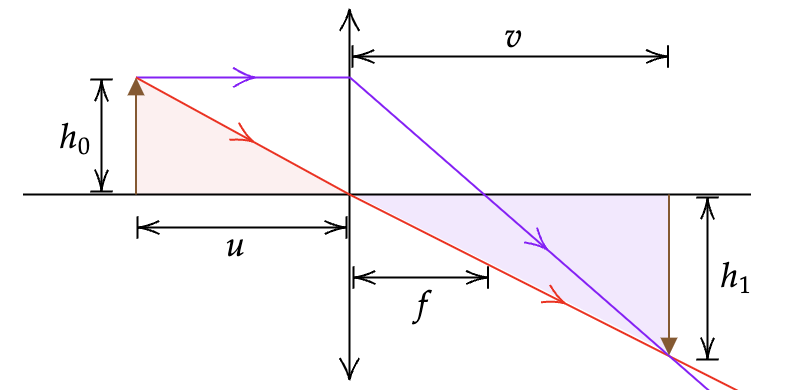
\includegraphics[width=0.7\linewidth]{assets/nxcu3489f43.png}
    \end{figure}
\end{frame}

\begin{frame}{}
    \begin{figure}
        \centering
        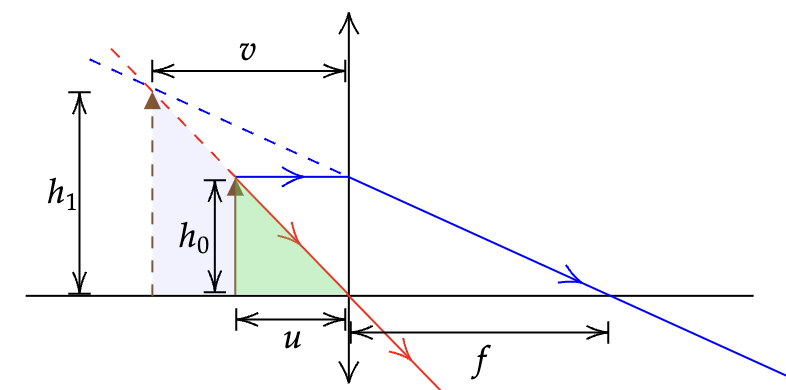
\includegraphics[width=0.7\linewidth]{assets/c82nu9238d.png}
    \end{figure}
    \begin{figure}
        \centering
        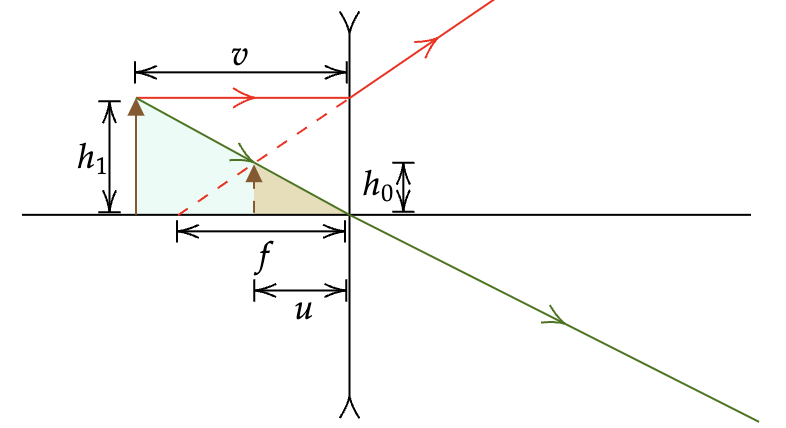
\includegraphics[width=0.7\linewidth]{assets/wedcnu89u34.png}
    \end{figure}
\end{frame}

\begin{eg}
    現用一放大鏡閱讀書上的小字。書和放大鏡距離 3 cm 且放大率為 3 。求小字的像和書之間的距離。\\
    A magnifying glass is begin used to read small characters in a book. The distance between the book and the magnifying glass is 3 cm, and the magnification is 3. Calculate the distance between the small characters and the book.
    \begin{tasks}
        \task \qty{1}{cm}
        \task \qty{3}{cm}
        \task \qty{6}{cm}
        \task \qty{9}{cm}
    \end{tasks}
\end{eg}

\begin{frame}{透鏡公式Lens formula}
    \begin{alertblock}
        {透鏡公式Lens formula}
        \begin{equation}
            \frac{1}{u}+\frac{1}{v}=\frac{1}{f}
        \end{equation}
    \end{alertblock}
    \renewcommand{\arraystretch}{3.2}
    \begin{table}
        \centering
        \begin{tabular}{c||c|c}
            % \hline
            $u$ & \makecell[l]{物距(物體與光心之間的距離) \\object distance (distance bet-\\ween object and optical centre)} & \makecell[l]{總是正號:($+$)\\always positive: ($+$)}\\
            \hline
            $v$ & \makecell[l]{像距(成像與光心之間的距離) \\image distance (distance bet-\\ween image and optical centre)} & \makecell[l]{實像real image: ($+$)\\虛像virtual image: ($-$)}\\
            \hline
            $f$ & \makecell[l]{焦距(焦點與光心之間的距離) \\focal length (distance between\\focus and optical centre)} & \makecell[l]{凸透鏡convex lens: ($+$)\\凹透鏡concave lens: ($-$)}\\
            % \hline
        \end{tabular}
        % \caption{Caption}
        \label{tab:my_label}
    \end{table}
\end{frame}

\begin{frame}{透鏡公式Lens formula}

    \renewcommand{\arraystretch}{2.15}
    \begin{longtable}{|>{\hspace{0pt}}m{0.192\linewidth}|>{\hspace{0pt}}m{0.079\linewidth}|>{\hspace{0pt}}m{0.079\linewidth}|>{\hspace{0pt}}m{0.233\linewidth}|>{\hspace{0pt}}m{0.23\linewidth}|}
        \cline{2-5}
        \multicolumn{1}{>{\hspace{0pt}}m{0.192\linewidth}|}{} & \multirow{2}{0.079\linewidth}{\hspace{0pt}\hspace{.5cm}$f$} & \multirow{2}{0.079\linewidth}{\hspace{0pt}\hspace{.5cm}$u$} & \multicolumn{2}{>{\hspace{0pt}}m{0.463\linewidth}|}{\hspace{2.3cm}$v$} \\*
        \cline{4-5}
        \multicolumn{1}{>{\hspace{0pt}}m{0.192\linewidth}|}{} &                                                             &                                                             & \makecell[l]{實像                                                        \\real image} & \makecell[l]{虚像\\virtual image}                          \endfirsthead
        \hline
        \makecell{凸透鏡                                                                                                                                                                                                                                              \\convex lens}                                               & \makecell{$+$}                                        & \makecell{$+$}                                        & \makecell{$+$}        & \makecell{$-$}                                    \\
        \hline
        \makecell{凹透鏡                                                                                                                                                                                                                                              \\concave lens}                                              & \makecell{$-$}                                        & \makecell{$+$}                                        & \makecell{N/A}          & \makecell{$-$}                                    \\
        \hline
    \end{longtable}
\end{frame}

\begin{eg}
    凸透鏡的焦距是 0.1 m,一個小物體放在它的主軸上距離它 0.2 m的地方。成像位于\\A convex lens of focal length 0.1 m has a small object placed 0.2 m from it on its principal axis. Where is the image?
    \begin{tasks}
        \task 在物體相同一邊 0.2 m 處。\\
        0.2 m on the same side as object.
        \task 在物體相同一邊 0.1 m 處。\\
        0.1 m on the same side as object.
        \task 在物體對面 0.2 m 處。\\0.2 m on the opposite side to object.
        \task 在物體對面 0.1 m 處。\\0.1 m on the opposite side to object.
    \end{tasks}
\end{eg}

\begin{eg}
    一位珠寶商正在使用一個焦距為30 mm的凸透鏡來觀察一顆鑽石。如果鑽石距離透鏡40 mm,像距是多少?\\A jeweler is using a converging lens of focal length 30 mm to view a diamond. If the diamond is placed 40 mm from the lens, what is the image distance?
    \begin{tasks}
        \task \qty{17}{mm}
        \task \qty{70}{mm}
        \task \qty{120}{mm}
        \task \qty{1200}{mm}
    \end{tasks}
\end{eg}



\begin{eg}
    一個凸透鏡形成了一個直立的成像,該成像距離物體28 cm 。成像的高度是物體高度的3倍。成像形成的位置在哪裡?\\A convex lens forms an erect image 28 cm from a real object. The image is 3 times as high as the object. Where is the image formed?
    \begin{tasks}
        \task 在物體相同一邊 21 cm 處。\\
        0.2 m on the same side as object.
        \task 在物體對面 21 cm 處。\\
        0.2 m on the opposite side to object.
        \task 在物體相同一邊 42 cm 處。\\
        0.1 m on the same side as object.
        \task 在物體對面 42 cm 處。\\
        0.1 m on the opposite side to object.
    \end{tasks}

\end{eg}

\begin{eg}
    一個凸透鏡形成了一個倒置的成像,該成像距離透鏡27 cm 。成像的高度是物體高度的兩倍。透鏡的焦距是多少?\\A convex lens forms an inverted image 27 cm from the lens. The image is twice as high as the object. What is the focal length of the lens?
    \begin{tasks}
        \task 3 cm
        \task 9 cm
        \task 15 cm
        \task 21 cm
    \end{tasks}
\end{eg}

\begin{eg}
    一個身高0.6 m 的男孩站在離門前30 cm 的地方。瑪麗透過門上的窺視孔看,該窺視孔有一個焦距為15 cm 的凹透鏡。男孩在瑪麗眼中看起來有多高?\\
    A 0.6 m tall boy is standing 30 cm in front of a door. Mary looks through a peep hole of the door that has a concave lens with focal length of 15 cm. How tall is the boy appearing to Mary?
    \begin{tasks}
        \task 10 cm
        \task 15 cm
        \task 20 cm
        \task 25 cm
    \end{tasks}
\end{eg}

\begin{frame}{遮住透鏡的一部分Covering part of the lens}
    \begin{figure}
        \centering
        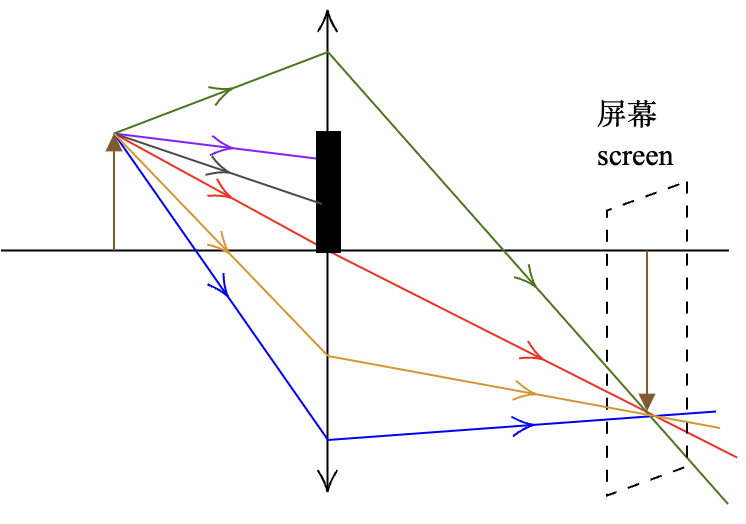
\includegraphics[width=0.75\linewidth]{assets/nud982u98u.png}


    \end{figure}
\end{frame}
\begin{frame}{遮住透鏡的一部分Covering part of the lens}
    \begin{itemize}
        \item 如果透鏡的一部分被遮住:\\If a lens is partly covered:
              \begin{itemize}
                  \item 透鏡折射的光線變少,成像變暗。\\Less light is refracted by the lens, the image becomes dimmer.
                  \item 成像的位置、大小和清晰度保持不變。\\The position, the size and the sharpness of the image remain unchanged.
              \end{itemize}
        \item 大尺寸的透鏡折射更多光線,成像會更亮。\\A lens with larger size refracts more light, the image is brighter.
    \end{itemize}
\end{frame}

\begin{frame}{遮住透鏡的一部分Covering part of the lens}
    \begin{figure}
        \centering
        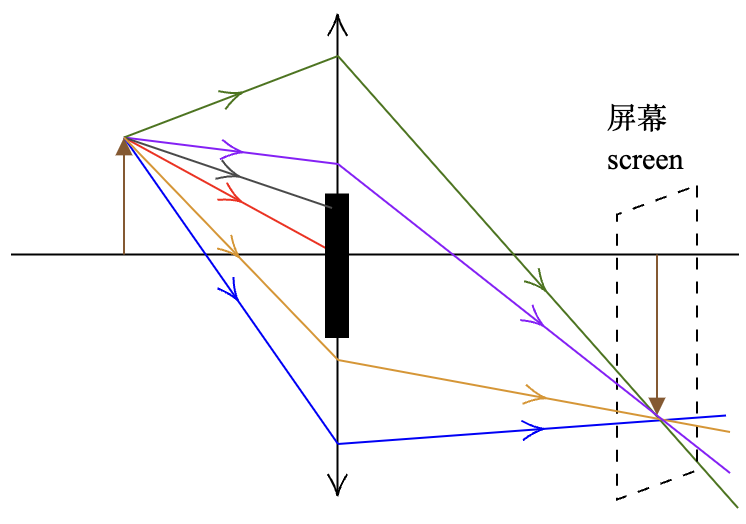
\includegraphics[width=0.75\linewidth]{assets/x89n9u92382.png}

        \caption{擋住中間也不影響實像的完整性Covering the middle part does not affect the image formation either}

    \end{figure}
\end{frame}

\begin{frame}{假如是虛像If image is virtual...}
    \begin{figure}
        \centering
        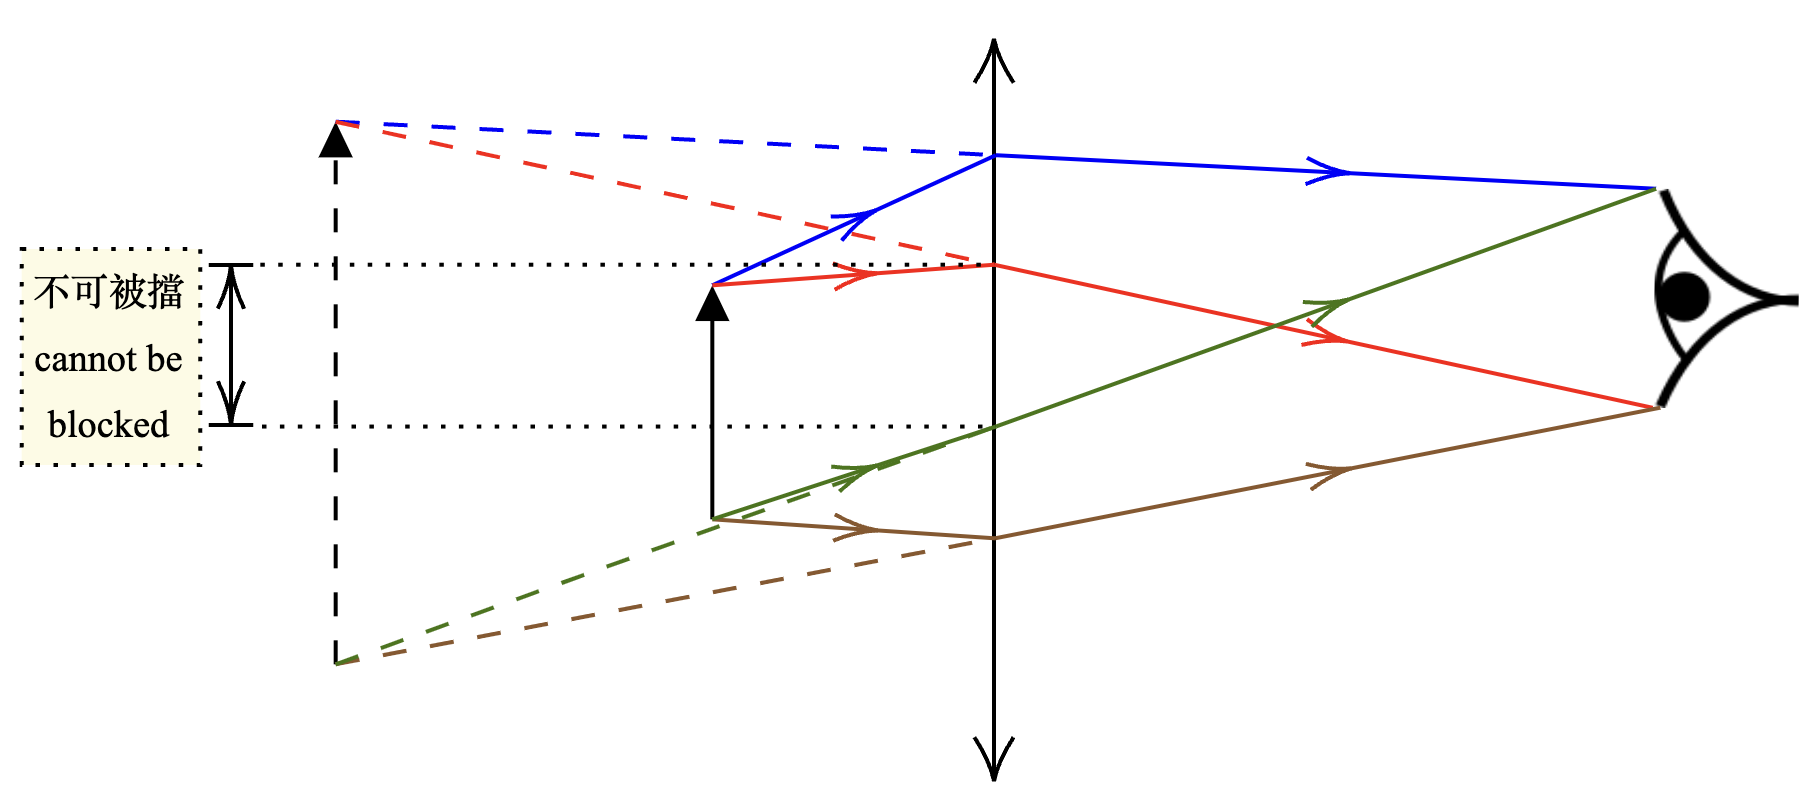
\includegraphics[width=1\linewidth]{assets/dun90du298n329.png}
        % \caption{假如是虛像If image is virtual...}
    \end{figure}
    \begin{itemize}
        % \setlength{}{}
        \item 因為觀察者的眼睛/相機有一定的尺寸大小,擋住某些部分的透鏡會影響觀察物件。\\Because the observer's eye/camera has a certain size, blocking certain parts of the lens will affect the observation of the object.
    \end{itemize}
\end{frame}

% \begin{frame}{假如是虛像If image is virtual...}

% \end{frame}


\begin{frame}{利用遠方事物尋找凸透鏡的焦距Finding focal length of a convex lens using distant objects}
    \begin{figure}
        \centering
        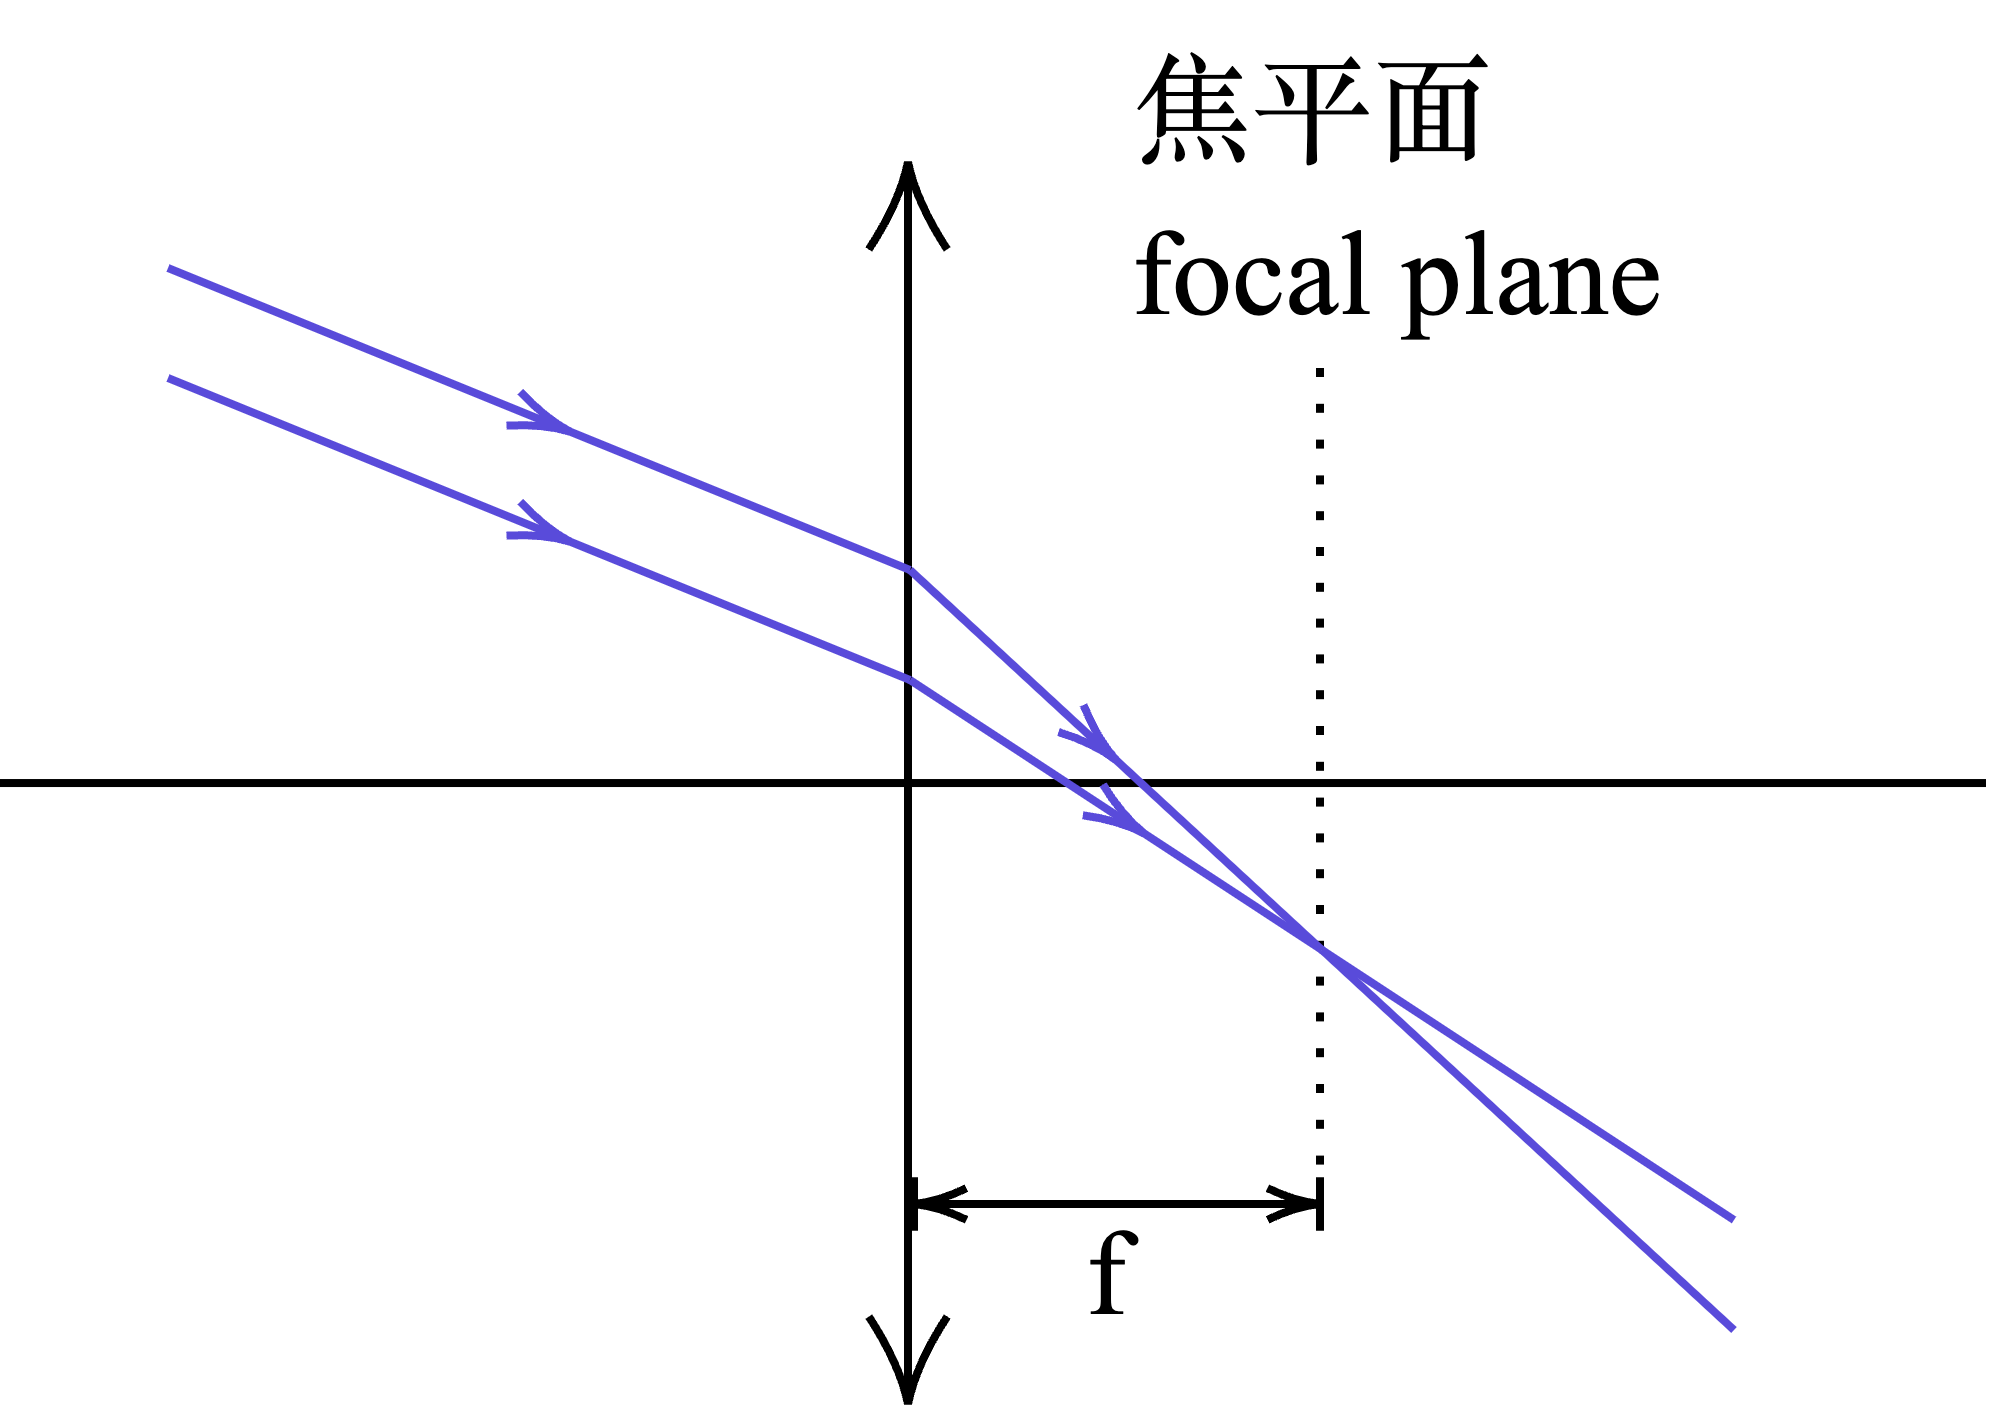
\includegraphics[width=0.7\linewidth]{assets/ddun2du8923.png}


    \end{figure}





\end{frame}

\begin{frame}{利用遠方事物尋找凸透鏡的焦距Finding focal length of a convex lens using distant objects}
    \begin{enumerate}
        \setlength{\itemsep}{.6em}
        \item 將透鏡朝向遠處的物體。\\Face the lens towards a distant object.
        \item 將清晰的成像投射到屏幕上。\\Capture the sharp image onto a screen.
        \item 用尺子測量透鏡和屏幕之間的距離,這個距離就是凸透鏡的焦距$f$。\\Measure the distance between the lens and the screen by a ruler. This distance is the focal length $f$ of the convex lens.
        \item 對於遠處的物體,在屏幕上形成的成像是實像、倒置和縮小的。\\For a distant object, the image formed on the screen is real, inverted and diminished.
    \end{enumerate}
\end{frame}

\begin{frame}{利用平面鏡尋找凸透鏡的焦距Finding focal length of a convex lens using a plane mirror}
    \begin{figure}
        \centering
        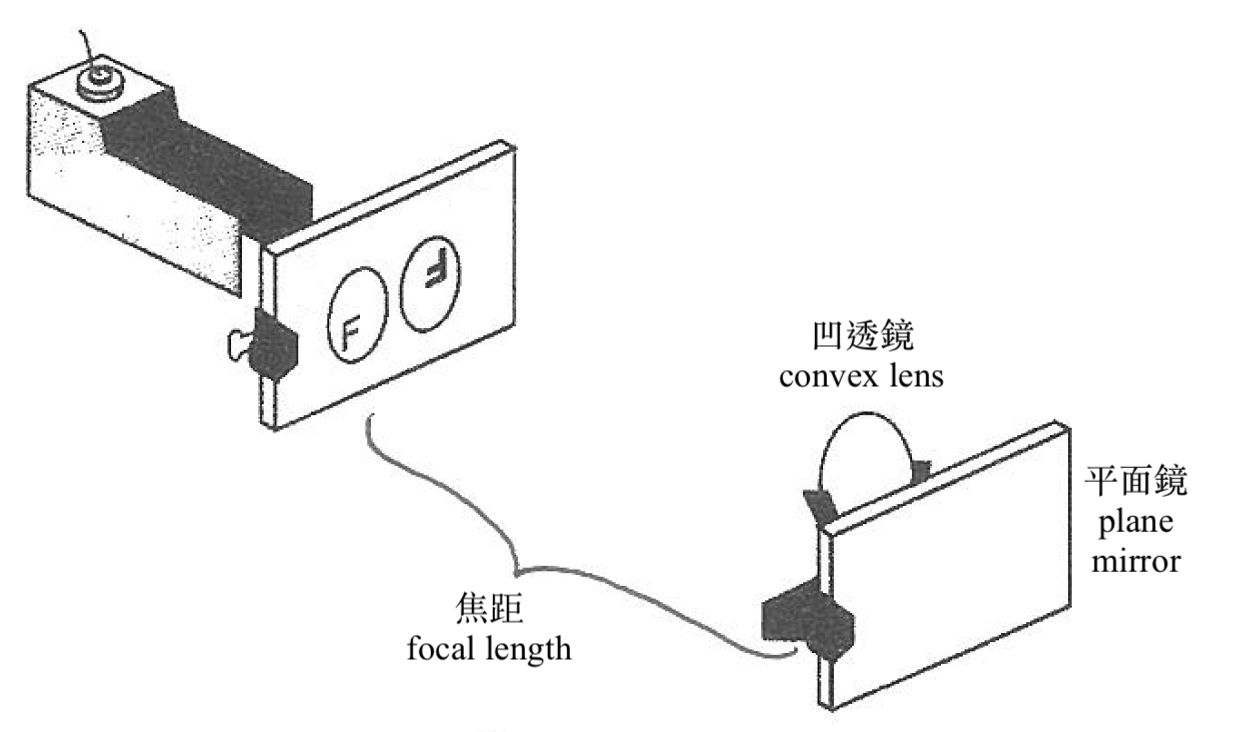
\includegraphics[width=0.75\linewidth]{assets/dd12cew8un9e8bew.png}


    \end{figure}
\end{frame}


\begin{frame}{利用平面鏡尋找凸透鏡的焦距Finding focal length of a convex lens using a plane mirror}
    \begin{figure}
        \centering
        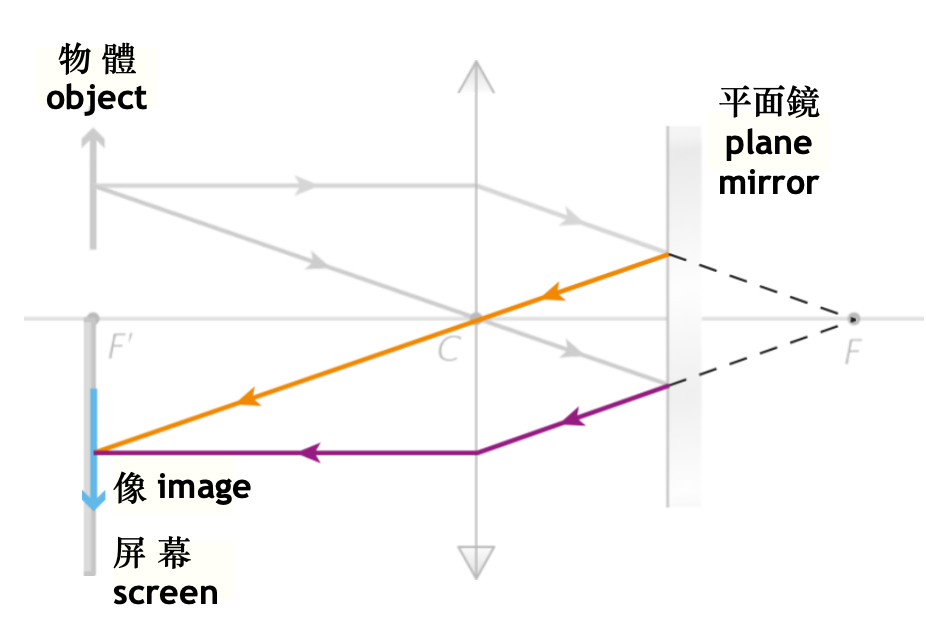
\includegraphics[width=0.75\linewidth]{assets/denu98u23.png}


    \end{figure}
\end{frame}

\begin{frame}{利用平面鏡尋找凸透鏡的焦距Finding focal length of a convex lens using a plane mirror}
    \begin{itemize}
        \item [] 簡化版Simplified version
    \end{itemize}
    \begin{figure}
        \centering
        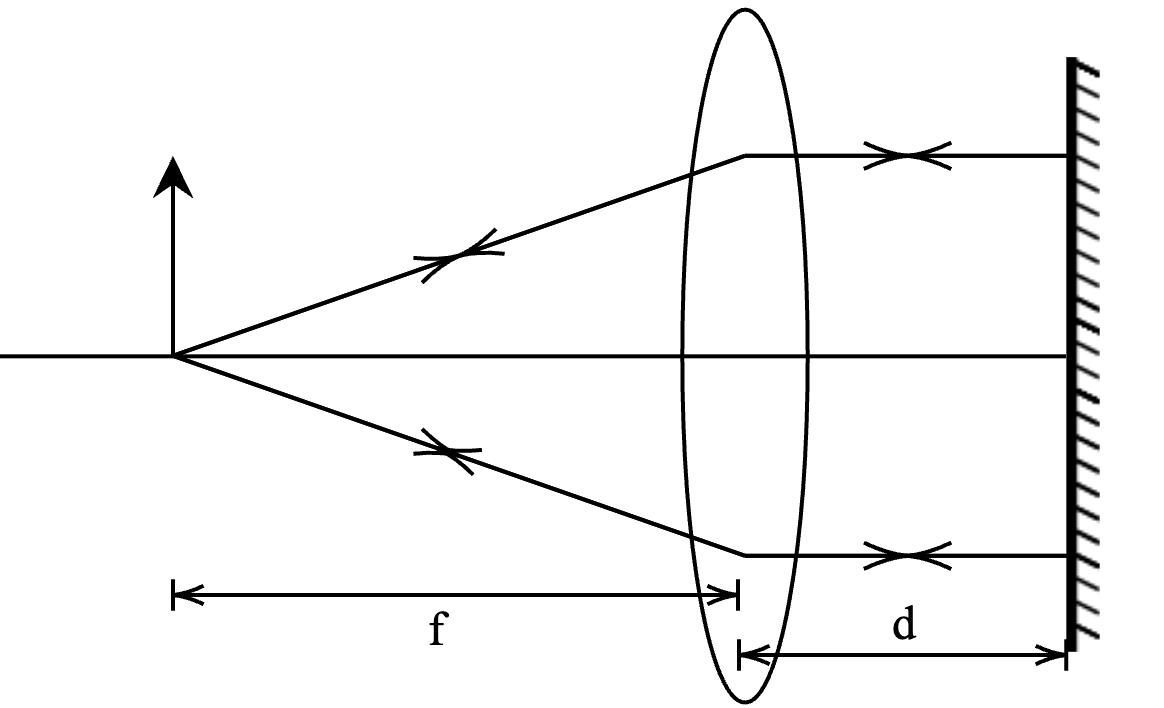
\includegraphics[width=0.75\linewidth]{assets/udhe08dnue8983.png}
    \end{figure}
\end{frame}

\begin{frame}{利用平面鏡尋找凸透鏡的焦距Finding focal length of a convex lens using a plane mirror}
    \begin{enumerate}
        \setlength{\itemsep}{.6em}
        \item 將一塊平面鏡垂直放置在一個凸透鏡後方。\\Place a plane mirror vertically behind a convex lens.
        \item 調整物體的位置,使成像與物體重合。\\Adjust the position of an object so that the image is coincident with the object.
        \item 測量物體和透鏡之間的距離。這就是透鏡的焦距。\\Measure the distance between the object and the lens. It is the focal length of the lens.
    \end{enumerate}
    \begin{itemize}
        \item [btw..] 調整透鏡和鏡子之間的距離 $d$不會影響結果。\\Changing the separation between the lens and the mirror $d$ does not affect the result.
    \end{itemize}
\end{frame}

\begin{eg}
    \begin{figure}
        \centering
        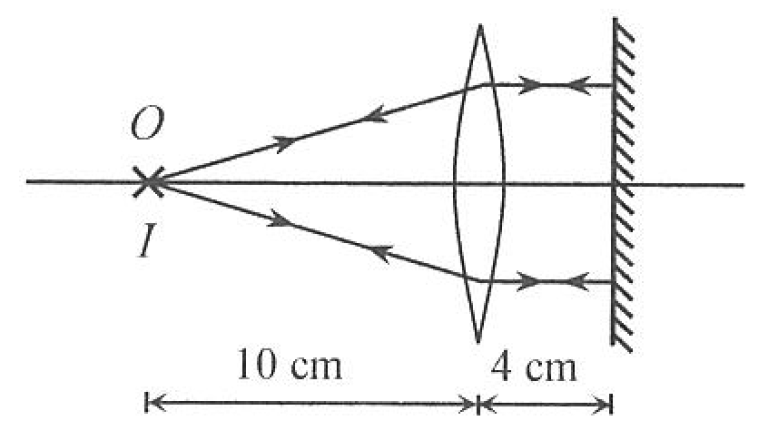
\includegraphics[width=0.5\linewidth]{assets/dnu983.png}
    \end{figure}
    上圖顯示物體$O$置於一凸透鏡和平面鏡之前,一像$I$成於物體所置的地方。下列各項敍述,哪些是正確的?When an object $O$ is placed in front of a convex lens and a plane mirror as shown above, an image $I$ is formed at the same positions as the object. Which of the following statements is/are correct?

\end{eg}
\begin{eg}
    \begin{statements}[before-skip=.8em,after-item-skip=0em]
        \task $I$為實像。\\The image $I$ is real.
        \task 透鏡的焦距為 \qty{10}{cm}。\\The focal length of lens is \qty{10}{cm}.
        \task 若把透鏡和平面鏡之間的距離改為 \qty{2}{cm},成像$I$的位置維持不變。\\If the distance between the lens and the plane mirror is changed to \qty{2}{cm}, the position of the image $I$ would remain unchanged.
    \end{statements}
    \begin{tasks} [before-skip=0em,after-item-skip=0.2em]
        \task 只有(1) \tab (1) only
        \task 只有(3) \tab (3) only
        \task 只有(1)和(2) \tab (1) and (2) only
        \task (1), (2) 和 (3)\tab (1), (2) and (3)
    \end{tasks}
\end{eg}

\begin{eg}
    \begin{figure}
        \centering
        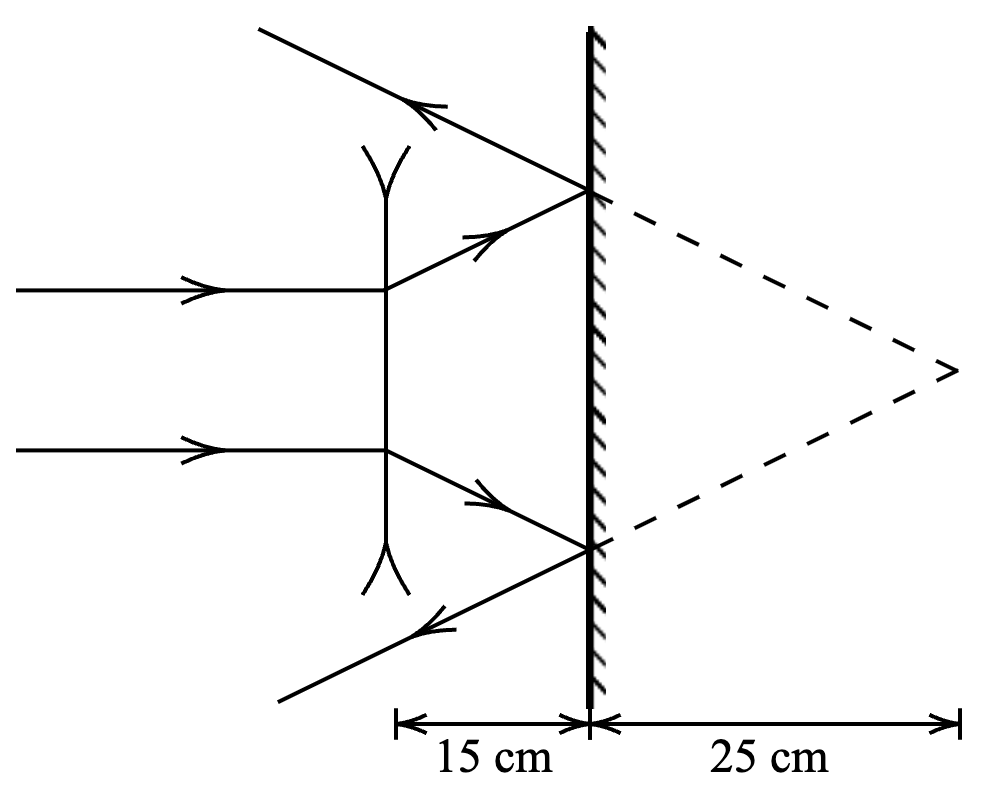
\includegraphics[width=0.5\linewidth]{assets/n8xu1980d23x23.png}
    \end{figure}
    一束平行光線通過凹透鏡並被平面鏡反射,如上圖所示。反射的光束似乎從點X散開。透鏡的焦距是多少?\\
    A beam of parallel light passes through a concave lens and is reflected by a plane mirror as shown in the above diagram. The reflected beam seems to diverge from the point X. The focal length of the lens is
\end{eg}
\begin{eg}
    \begin{tasks}
        \task 10 cm
        \task 15 cm
        \task 25 cm
        \task 40 cm
    \end{tasks}
\end{eg}

\begin{frame}{利用透鏡公式尋找凸透鏡的焦距Finding focal length of a convex lens using a lens formula}
    \begin{figure}
        \centering
        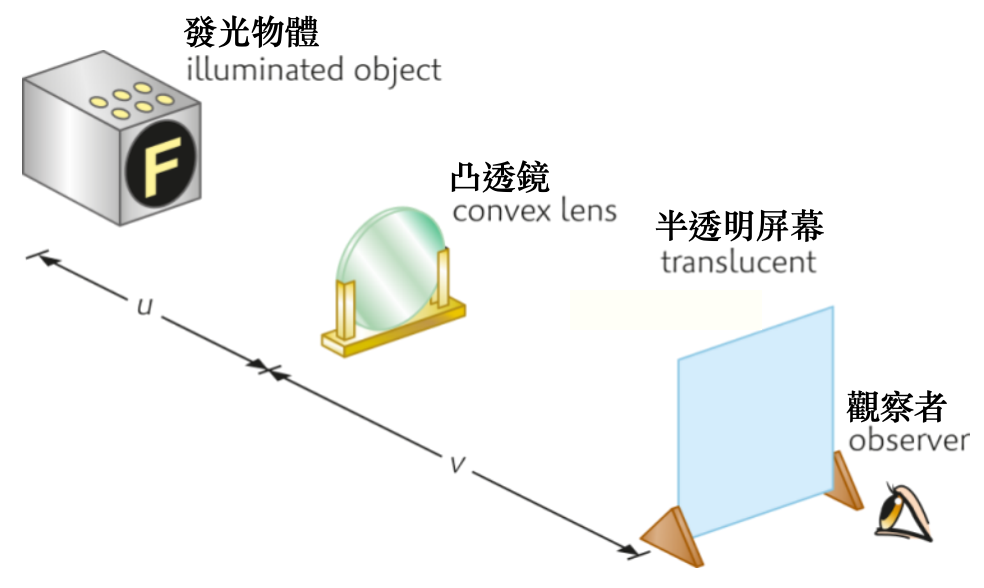
\includegraphics[width=1\linewidth]{assets/xu89n32r2r2frf.png}
    \end{figure}

\end{frame}

\begin{frame}{利用透鏡公式尋找凸透鏡的焦距Finding focal length of a convex lens using a lens formula}
    \begin{itemize}
        \item 將一個被照亮的物體放在凸透鏡後面。\\Place an illuminated object behind the convex lens.
        \item 調整放在凸透鏡前方的屏幕位置,以捕捉清晰的成像。\\Adjust the position of the screen placed in front of the convex lens to capture the sharp image.
        \item 用尺測量物距 $u$ 和像距 $v$。\\Measure the object distance $u$ and the image distance $v$ using a ruler.
        \item 重複上述步驟,獲取不同的 $u$ 和 $v$ 值。\\Repeat the above procedure to obtain different values of $u$ and $v$.
        \item 繪製一個合適的圖表,以找到焦距。\\Plot a suitable graph to find the focal length.
    \end{itemize}
\end{frame}

\begin{frame}{利用透鏡公式尋找凸透鏡的焦距Finding focal length of a convex lens using a lens formula}
    \begin{columns}
        \column{.5\textwidth}
        \begin{figure}
            \centering
            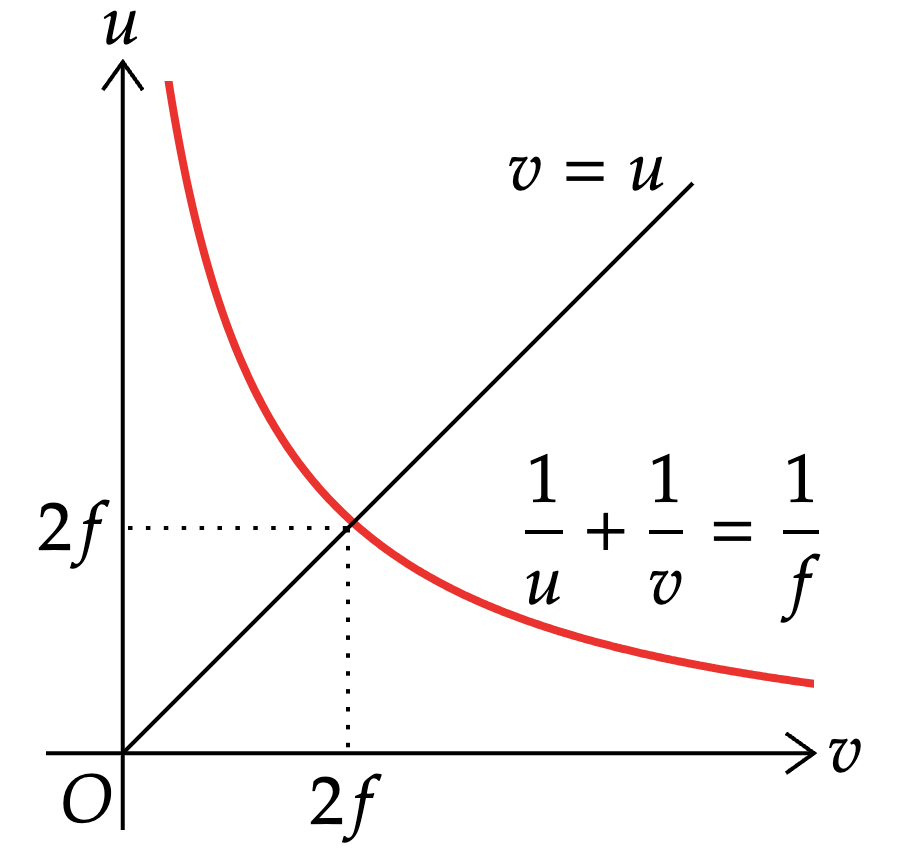
\includegraphics[width=\linewidth]{assets/dun98d89382d32.png}
        \end{figure}
        \column{.5\textwidth}
        \begin{figure}
            \centering
            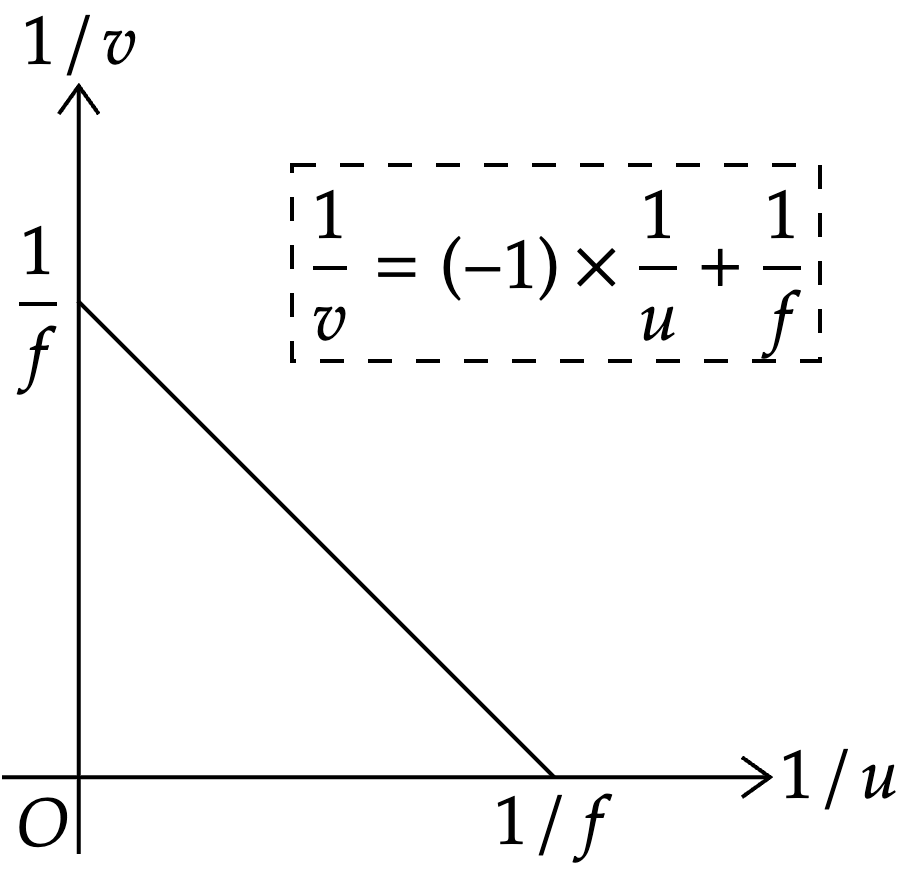
\includegraphics[width=\linewidth]{assets/dqwdqwjddge.png}
        \end{figure}
    \end{columns}
\end{frame}

\begin{eg}
    一學生利用圖 (a) 的裝置研究凸透鏡中物距 $u$ 和像距 $v$ 的關係。圖 (b) 顯示 $1/v$ 對 $1/u$ 的關
    係線圖。如果透鏡以另一塊焦距較短的凸透鏡取代,會得出以下哪一幅關係線圖 (以虛線表示) ?\bigskip
    \begin{columns}
        \column{.6\textwidth}
        \begin{figure}
            \centering
            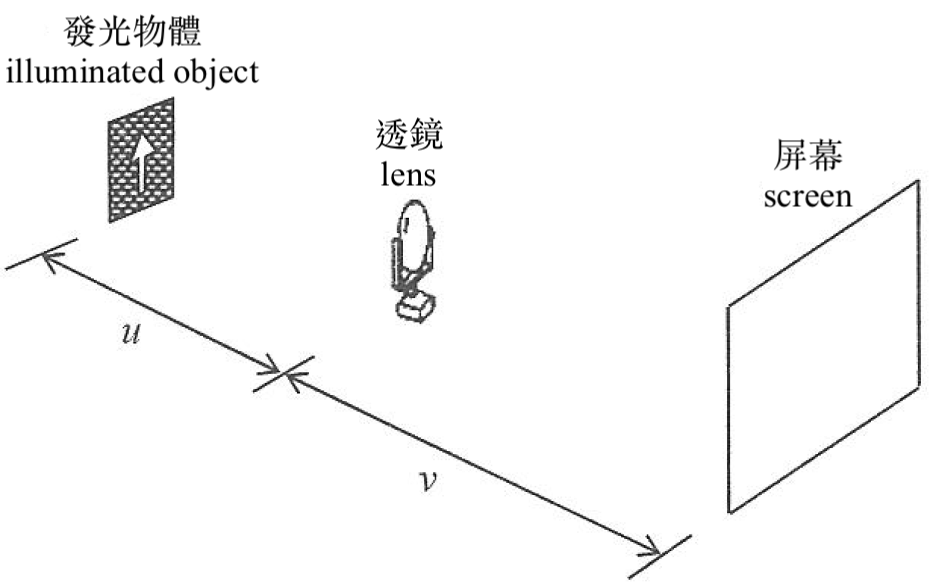
\includegraphics[width=\linewidth]{assets/d980un82dun8923d23.png}
            \caption{(a)}
        \end{figure}
        \column{.4\textwidth}
        \begin{figure}
            \centering
            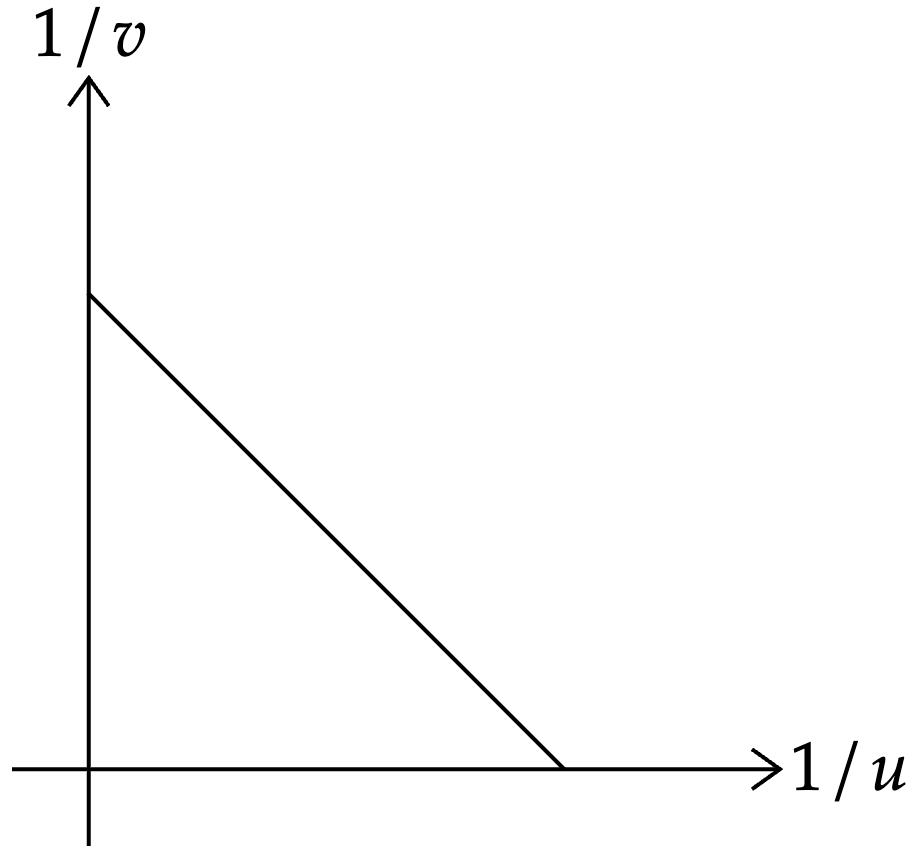
\includegraphics[width=\linewidth]{assets/dm90j2d3.png}
            \caption{(b)}
        \end{figure}
    \end{columns}
\end{eg}
\begin{eg}
    A student uses the set-up in Figure (a) to study the relationship between the object distance $u$ and the image distance $v$ of a convex lens. A graph of $1/v$ against $1/u$ is plotted in Figure (b). If the lens is replaced by another convex lens of shorter focal length, which of the following graphs (in dotted lines) would be obtained?
    \begin{columns}
        \column{.6\textwidth}
        \begin{figure}
            \centering
            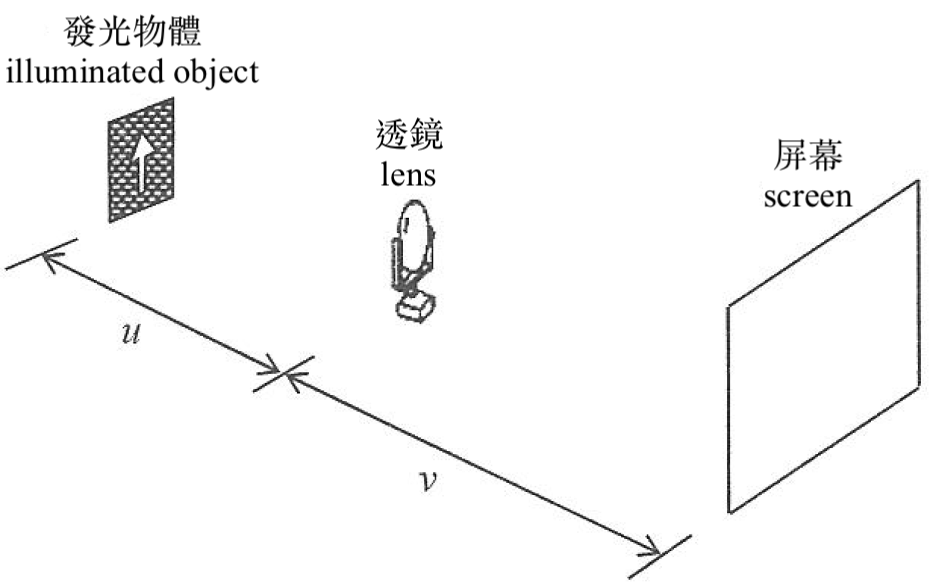
\includegraphics[width=\linewidth]{assets/d980un82dun8923d23.png}
            \caption{(a)}
        \end{figure}
        \column{.4\textwidth}
        \begin{figure}
            \centering
            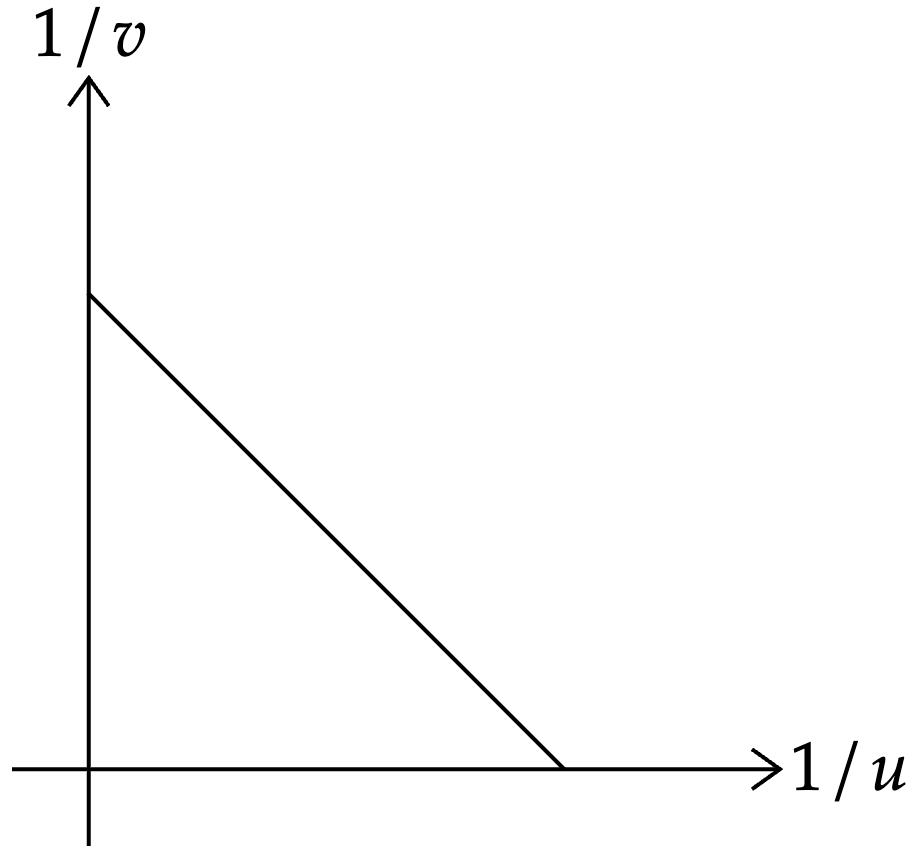
\includegraphics[width=\linewidth]{assets/dm90j2d3.png}
            \caption{(b)}
        \end{figure}
    \end{columns}
\end{eg}
\begin{eg}
    \begin{tasks}[item-indent=2em,label-offset=0em,before-skip=.3em,after-item-skip=.5em](2)
        \task
        \begin{figure}
            \centering
            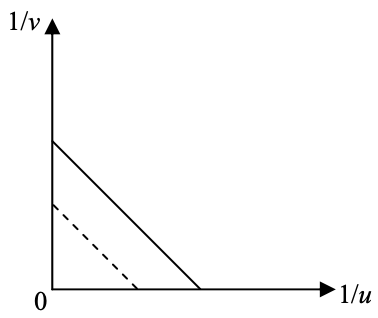
\includegraphics[width=0.7\linewidth]{assets/dun982393.png}
        \end{figure}
        \task
        \begin{figure}
            \centering
            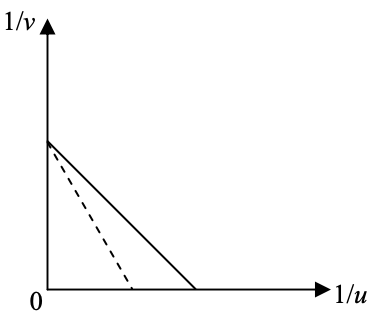
\includegraphics[width=0.7\linewidth]{assets/ddewcwcwcwcww.png}
        \end{figure}
        \task
        \begin{figure}
            \centering
            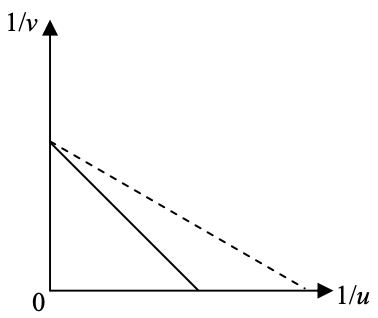
\includegraphics[width=0.7\linewidth]{assets/ewwewefwfqweqf.png}
        \end{figure}
        \task
        \begin{figure}
            \centering
            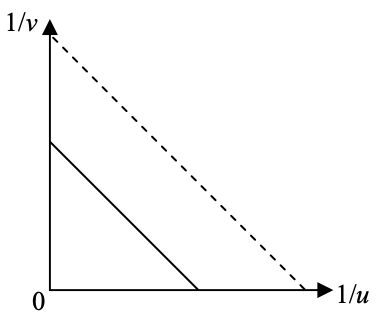
\includegraphics[width=0.7\linewidth]{assets/deqdededqewdeqe.png}
        \end{figure}
    \end{tasks}
\end{eg}



\begin{frame}{假如焦距改變If focal length changes}
    \begin{figure}
        \centering
        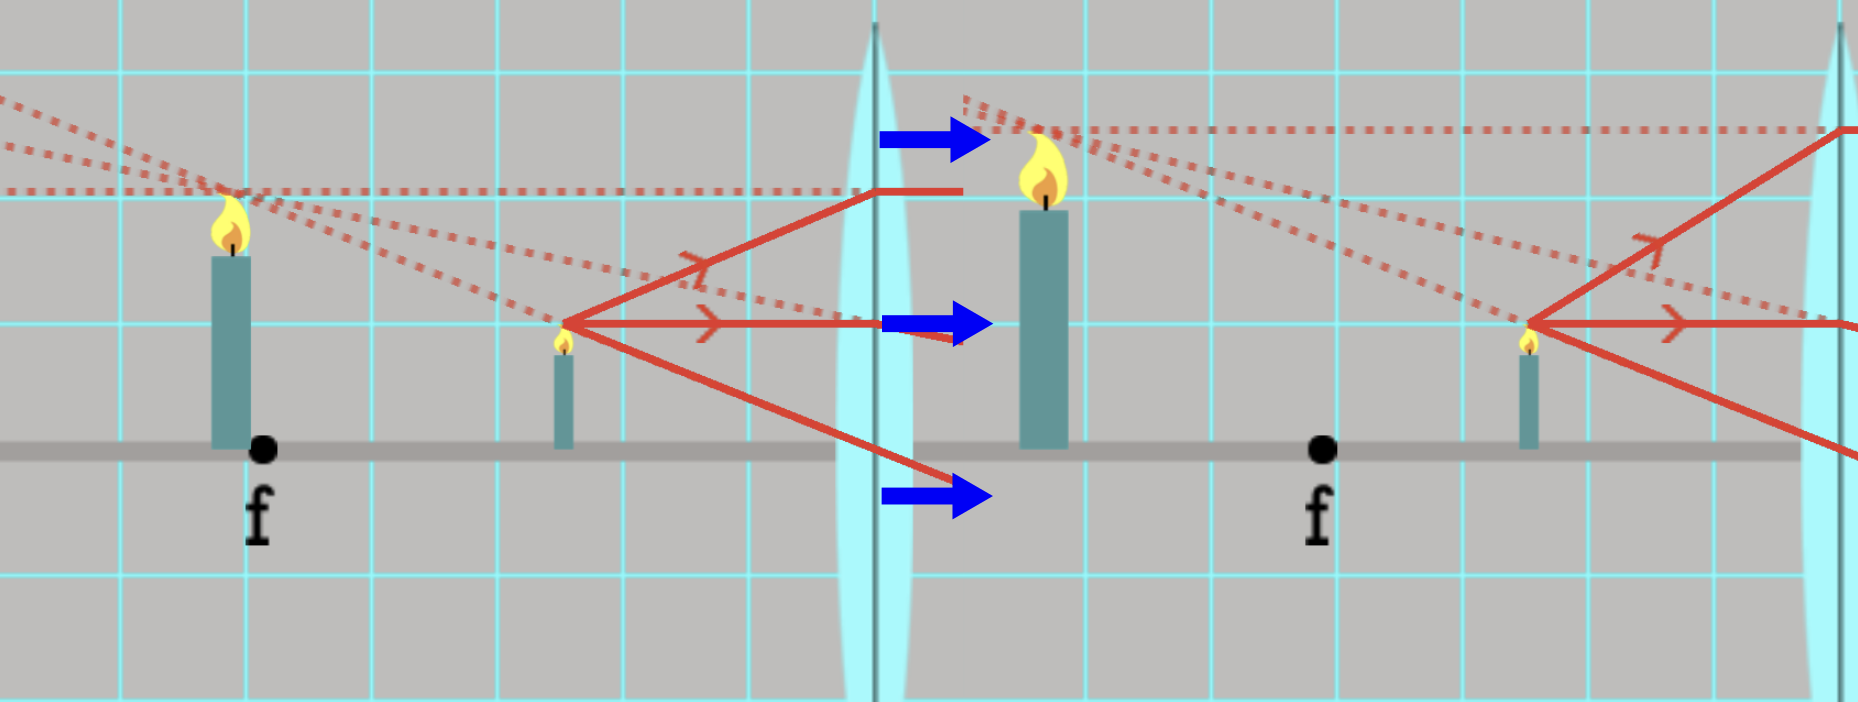
\includegraphics[width=1\linewidth]{assets/x9n80ue213e.png}
    \end{figure}
\end{frame}

\begin{frame}{假如焦距改變If focal length changes}
    \begin{figure}
        \centering
        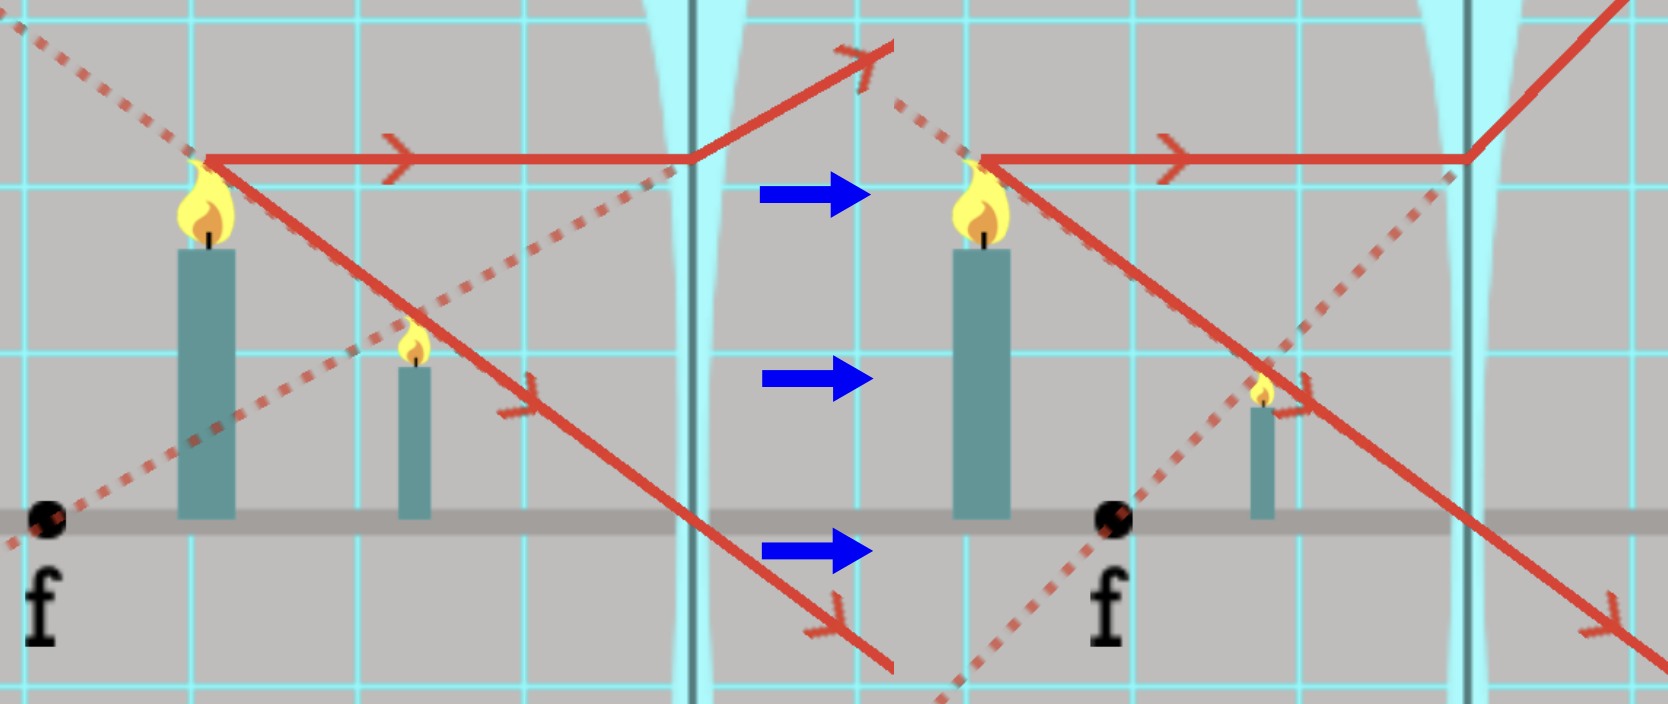
\includegraphics[width=1\linewidth]{assets/n9du82u8e.png}
    \end{figure}
\end{frame}

\begin{eg}
    一物體放置在凹透鏡前,成像與透鏡的距離為$v$。若使用另一折射率更大的凹透鏡取代。$v$值的改變是\\
    An object is placed in front of a concave lens, the distance between the image and the lens is denoted as $v$. If we replace the concave lens with another lens having a higher refractive index, $v$ would be...
    \begin{statements}
        \task 增加\\increased
        \task 減少\\decreased
        \task 無從判斷\\undetermined
    \end{statements}
\end{eg}

\begin{eg}
    一物體放置在凹透鏡前,成像與透鏡的距離為$v$。若使用另一焦距相同的凸透鏡取代。$v$值的改變是\\
    An object is placed in front of a concave lens, the distance between the image and the lens is denoted as $v$. If we replace the concave lens with a convex lens having same focal length, $v$ would be...
    \begin{statements}
        \task 增加\\increased
        \task 減少\\decreased
        \task 無從判斷\\undetermined
    \end{statements}
\end{eg}


\end{document}